\documentclass[12pt, a4paper, reqno, oneside]{report}
\usepackage[utf8]{vietnam}
\usepackage{amsmath,amsxtra,amssymb,latexsym, amscd,amsthm}
\usepackage{indentfirst}
\usepackage{color}
\usepackage{fancyhdr}
\usepackage[mathscr]{eucal}
\usepackage{amsfonts}
\usepackage{amssymb}
\usepackage[unicode]{hyperref}
\usepackage{graphicx}
\usepackage{graphics} % thư viện để hiển thị ảnh
\usepackage{caption} % thư viện để đặt caption
\usepackage{booktabs} % thư viện để vẽ table
\usepackage{hyperref} % thư viện để link tới các chương
\usepackage{titledot}

\titlename{Chương}
\usepackage[left=3cm,right=2cm,top=2cm,bottom=2cm]{geometry}

\usepackage[backend=bibtex,style=numeric,natbib=true]{biblatex}
\bibliography{ref}

\setcounter{secnumdepth}{5}  
\setcounter{tocdepth}{2}   

\renewcommand{\theequation}{\arabic{chapter}.\arabic{section}.\arabic{equation}}
\newtheorem{lemma}{\bf Bổ đề}[section]
\newtheorem{theorem}{\bf Định lý}[section]
\newtheorem{proposition}{\bf Mệnh đề}[section]
\newtheorem{corollary}{\bf Hệ quả}[section]
\newtheorem{definition}{\bf Định nghĩa}[section]
\newtheorem{remark}{\bf Chú ý}[section]

%\usepackage{fancyhdr}
\setlength{\headheight}{40pt}
\pagestyle{fancy}
\fancyhead{} % clear all header fields
\graphicspath{ {img/} }
\fancyhead[L]{
	\begin{tabular}{rl}
		\begin{picture}(25,15)(0,0)
		\put(0,-8){
\includegraphics[width=9mm, height=8mm]{img/logo.png}}
		\end{picture}&
		\begin{tabular}{l}
			\textbf{\bf \ttfamily Trường Đại Học Bách Khoa TP.Hồ Chí Minh}\\
			\textbf{\bf \ttfamily Khoa Khoa Học \& Kỹ Thuật Máy Tính}
		\end{tabular} 	
	\end{tabular}
}
\fancyhead[R]{
	\begin{tabular}{l}
		\tiny \bf \\
		\tiny \bf 
\end{tabular}  }
\setlength{\headheight}{30pt}
\fancyfoot{} % clear all footer fields
\fancyfoot[L]{\bf \ttfamily Luận văn tốt nghiệp}
\fancyfoot[R]{\bf \ttfamily Trang {\thepage}}
\renewcommand{\headrulewidth}{0.3pt}
\renewcommand{\footrulewidth}{0.3pt}

\begin{document}
	\makeatletter
	\renewcommand{\ps@myheadings}{
		\renewcommand{\@oddhead}{\textsf{Luận văn tốt nghiệp - công nghệ thông tin}\hfil\textrm{\thepage}}
		\renewcommand{\@oddfoot}{\textsf{Phan Minh Cường, Khoa Khoa học \& Kỹ thuật máy tính}\hfil}
	}
	
	%+ Page style
	\newpage
	
\begin{titlepage}
\centerline{\fontsize{15}{15}\bf ĐẠI HỌC QUỐC GIA TP.HCM}
\centerline{\fontsize{15}{15}\bf TRƯỜNG ĐẠI HỌC BÁCH KHOA}
\centerline{\fontsize{15}{15}\bf KHOA KHOA HỌC \& KỸ THUẬT MÁY TÍNH}
\begin{center}
	\begin{figure}[htp]
		\begin{center}
			
\includegraphics[scale=0.1]{img/logo}
		\end{center}
	\end{figure}
\end{center}
\centerline{\fontsize{15}{15}\bf LUẬN VĂN TỐT NGHIỆP ĐẠI HỌC}
\vspace*{2cm}
\centerline{\Large\bf NGHIÊN CỨU \& XÂY DỰNG CÔNG CỤ}
\vspace*{0.5cm}
\centerline{\Large\bf HỖ TRỢ VÀ ĐÁNH GIÁ HỌC VIÊN TRÊN MOODLE}
\vskip 0.5cm
\hskip 4.9cm {———————————————}
\vskip 1.5cm
\hskip3cm{\fontsize{15}{15}\bf HỘI ĐỒNG:}
\vskip 0.5cm
\hskip3cm{\fontsize{15}{15}\bf GVHD: PGS.TS THOẠI NAM}
\vskip 0.5cm
\hskip3cm{\fontsize{15}{15}\bf GVPB: ...}
\vskip 0.5cm
\centerline{———————o0o———————}
\vskip 0.5cm
\hskip3cm{\fontsize{15}{15}\bf SVTH 1: PHAN MINH CƯỜNG (1510381)}
\vskip 0.5cm
\hskip3cm{\fontsize{15}{15}\bf SVTH 2: HUỲNH BẢO HIẾU (1511004)}
\vfill
\centerline{\bf TP.HỒ CHÍ MINH, 6/2019}
\end{titlepage}
	
	\newpage
	\centerline{\bf \large\MakeUppercase{Lời cam đoan}}

\vspace{20pt}

Nhóm chúng em xin cam đoan đây là công trình nghiên cứu độc lập của nhóm với sự hướng dẫn của PGS. TS. Thoại Nam và ThS. Diệp Thanh Đăng, tất cả các nguồn tài liệu đã được công bố đầy đủ và tất cả nội dung của Luận văn này là trung thực. Nếu không đúng như đã nêu trên, chúng em xin hoàn toàn chịu trách nhiệm về đề tài của mình.

\begin{flushright}
	{\it TP. Hồ Chí Minh, tháng 06 năm 2019}
	
	Sinh viên cam đoan \hskip 2cm\quad
	
	\vskip 1cm
	{\bf Phan Minh Cường, Huỳnh Bảo Hiếu} \quad\ 
\end{flushright}

	
	\newpage
	\centerline{\bf \large\MakeUppercase{Lời cảm ơn}}

\vspace{20pt}

Trước khi trình bày nội dung của luận văn, nhóm chúng em xin gửi lời cảm ơn sâu sắc tới PGS.TS Thoại Nam, ThS. Diệp Thanh Đăng những người đã tận tình hướng dẫn để nhóm có thể hoàn thành luận văn này.

Nhóm cũng xin cảm ơn tới toàn thể các thầy cô trong khoa Khoa học \& Kỹ thuật máy tính Đại Học Bách Khoa, Đại Học Quốc Gia TP.HCM đã dạy bảo chúng em tận tình trong suốt quá trình học tập tại trường.

Đồng thời, chúng em cũng xin được gửi lời cảm ơn chân thành tới gia đình, bạn bè đã luôn bên cạnh, cổ vũ, động viên chúng em trong suốt quá trình học tập và thực hiện luận văn tốt nghiệp. 

Một lần nữa, chúng em xin chân thành cảm ơn! 

\begin{flushright}
	{\it TP.Hồ Chí Minh, tháng 06 năm 2019}\\

	Sinh viên \hskip 2.5cm\quad
	
	\vskip 1cm
	{\bf Phan Minh Cường, Huỳnh Bảo Hiếu} \quad\ 
\end{flushright}
	
	\newpage
	\centerline{\bf \large\MakeUppercase{Tóm tắt luận văn}}
\vspace{20pt}

Trong thời đại công nghệ hiện đại ngày nay, việc sử dụng Internet để học tập trực tuyến đang là xu hướng của hầu hết các trung tâm giảng dạy hay các trường đại học ở nước ta. Hệ thống E-Learning giúp cho học viên tương tác với môi trường học tập một cách chủ động.

Nắm bắt được xu hướng của việc học tập hiện nay, nhóm quyết định thực hiện đề tài nhằm xây dựng một công cụ nhằm hỗ trợ, đánh giá từng cá nhân trong mỗi khóa học trực tuyến.

Trong phạm vi luận văn, nhóm sẽ dựa trên hệ thống quản lý học tập (Learning Management System - LMS) Moodle, một hệ thống cung cấp đầy đủ các công cụ để tạo ra một khóa học online để phân tích và xây dựng một công cụ mới nhằm hỗ trợ và đánh giá năng lực của học viên trong mỗi khóa học. Công cụ có tên là E-Learning Help and Assess Tool (EHAT).

Luận văn tập trung làm rõ một số vấn đề sau:

\begin{itemize}
	\item Nội dung cơ bản về hệ thống quản lý đào tạo Moodle.
	\item Trình bày tóm tắt các kiến thức liên quan.
	\item Cách xây dựng một plugin trên nền tảng Moodle.
	\item Hiện thực, kết quả và đánh giá công cụ EHAT.
\end{itemize}

Thông qua đề tài nhóm đã rút ra nhiều bài học hữu ích cũng như đã cải thiện hơn về kỹ năng phân tích, giải quyết vấn đề. Tất cả đều là những hành trang tốt đẹp hỗ trợ cho chúng em khi bắt đầu tham gia vào môi trường làm việc thực tế sau này.
	
	\newpage
	\tableofcontents
	
	\newpage
	{\huge\bf Danh mục từ viết tắt} 
	
	\begin{center}
		\begin{table}[!htp]
			\centering
			\begin{tabular}{|c|c|}
				\hline 
				Tên cụ thể & Tên viết tắt \\ 
				\hline 
				E-learning Help And Assess Tool & EHAT \\ 
				\hline 
				Giáo viên & GV \\ 
				\hline 
				Học sinh & HS \\ 
				\hline 
				Sinh viên & SV \\ 
				\hline 
				Học viên & HV \\ 
				\hline 
			\end{tabular}
			\label{bang}
		\end{table}
	\end{center}
	
	\newpage
	\listoftables
	
	\newpage
	\listoffigures

	\newpage
	\setcounter{chapter}{0}
\fontsize{13}{5}\selectfont
\chapter{Tổng quan về đề tài}
\section{Giới thiệu đề tài}
Trong thời đại công nghệ 4.0 hiện nay, việc học tập trực tuyến đối với mọi người càng trở nên phổ biến. Đã có rất nhiều trang đào tạo trực tuyến ở Việt Nam phục vụ cho việc học tập trực tuyến. Trong quá trình tìm hiểu về những trang đào tạo ấy chúng em đã rút ra được những vấn đề mà mình cần phải giải quyết trong phạm vi luận này đó là:

\begin{itemize}
	\item Người học có thể tận dụng khoảng thời gian tối thiểu để thu về được lượng kiến thức tối đa.
	\item Giáo viên có thể đánh giá được chi tiết từng cá nhân học viên trong học.
	\item Giáo viên đánh giá được mức độ hiệu quả của việc xây dựng bài giảng, bài kiểm tra trong khóa học của mình.
	\item Mô tả được thái độ cũng như là hành vi học tập của từng cá nhân học viên trong khóa học.
\end{itemize}

Để giải quyết những vấn đề trên nhóm đã quyết định xây dựng một công cụ chạy trên nền tảng Moodle có tên là E-learning Help And Assess Tool(EHAT) có những chức năng sau:

\begin{itemize}
	\item Về khóa học mẫu:
	\begin{itemize}
		\item Nội dung bài giảng ngắn gọn, dễ hiểu không gây nhàm chán.
		\item Có video giảng dạy.
		\item Có một hoặc nhiều bài kiểm tra đánh giá sau mỗi chương trong mỗi khóa học.
		\item Có bài kiểm tra tổng hợp
	\end{itemize}
	\item Về công cụ hỗ trợ đánh giá (EHAT):
	\begin{itemize}
		\item Biểu đồ radar đánh giá chi tiết điểm của từng sinh viên trong mỗi khóa học.
		\item So sánh biểu đồ của hai sinh viên.
		\item Biểu đồ thống kê số lượt truy cập của sinh viên
		\item Biểu đồ phân phối lượt truy cập của từng sinh viên trong khóa học
		\item Bảng hỗ trợ giảng viên thêm tài liệu tham khảo
	\end{itemize}
\end{itemize}

\section{Lý do chọn đề tài}
Chắc hẳn trong chúng ta ai cũng đã từng trải qua giai đoạn ngồi trên ghế nhà trường và cảm nhận được những khó khăn nhất định trong quá trình học tập của mình như:
\begin{itemize}
	\item Không linh hoạt về thời gian.
	\item Tốn kém hơn về chi phí và công sức.
	\item Khó có lại kiến thức nếu vắng một buổi học.
	\item Sự tương tác giữa học sinh, sinh viên với giáo viên thấp.
	\item Đánh giá kết quả thông qua các bài kiểm tra.
	\item Không đánh giá được thái độ học tập của từng sinh viên trong quá trình học tập trực tuyến
\end{itemize}
Nắm bắt được những khó khăn đó cùng với niềm mong muốn tạo ra một khóa học trực tuyến nhằm để tạo điều kiện thuận lợi hơn trong việc giảng dạy cũng như đánh giá năng lực của học viên. Nhóm chúng em đã lựa chọn đề tài này làm đề tài để nghiên cứu và thực hiện.

\section{Mục tiêu của đề tài}
\begin{itemize}
	\item Xây dựng thành công công cụ EHAT trên nền tảng Moodle để có thể đánh giá cũng như hỗ trợ được học viên trong suốt quá trình học tập trực tuyến.
	\item Công cụ tương thích với hầu hết các khóa học sử dụng nền tảng Moodle
	\item EHAT dễ dàng nâng cấp cũng như mở rộng trong tương lai.
\end{itemize}

\section{Phương pháp hiện thực đề tài}
Từ những mục tiêu đề ra cùng với việc sử dụng nền tảng Moodle để xây dựng công cụ. Nhóm chúng em quyết định xây dựng EHAT bằng ngôn ngữ lập trình PHP, MySQL và Apache làm server.

\section{Cấu trúc luận văn}
Bố cục của luận văn bao gồm các chương sau:
\begin{itemize}
	\item Chương 1: Tổng quan về đề tài. Chương này sẽ giới thiệu đề tài, lý do chọn đề tài, mục tiêu và phương pháp của đề tài.
	\item Chương 2: Chương này sẽ trình bày tóm tắt những kiến thức nền tảng liên quan đến quá trình xây dựng hệ thống.
	\item Chương 3: Phân tích hệ thống use case, database, những dạng biểu đồ sử dụng trong công cụ.
	\item Chương 4: Hiện thực và triển khai.
	\item Chương 5: Kết luận và hướng phát triển đề tài.
\end{itemize}
	
	\newpage
	\setcounter{chapter}{1}
\chapter{Kiến thức nền tảng}
\section{Giới thiệu về LMS \cite{lms}}
\subsection{LMS là gì?}
LMS là chữ viết tắt của Learing Management System, dịch ra tiếng Việt có nghĩa là Hệ thống quản lý học trực tuyến. Về bản chất đây là một phần mềm ứng dụng cho phép việc quản lý, vận hành hệ thống các tài liệu, hướng dẫn, theo dõi, báo cáo và cung cấp các công nghệ giáo dục điện tử (hay còn gọi là giáo dục trực tuyến E-Learning) cho các khóa học hay chương trình đào tạo.
\begin{center}
	\begin{figure}[htp]
		\begin{center}
			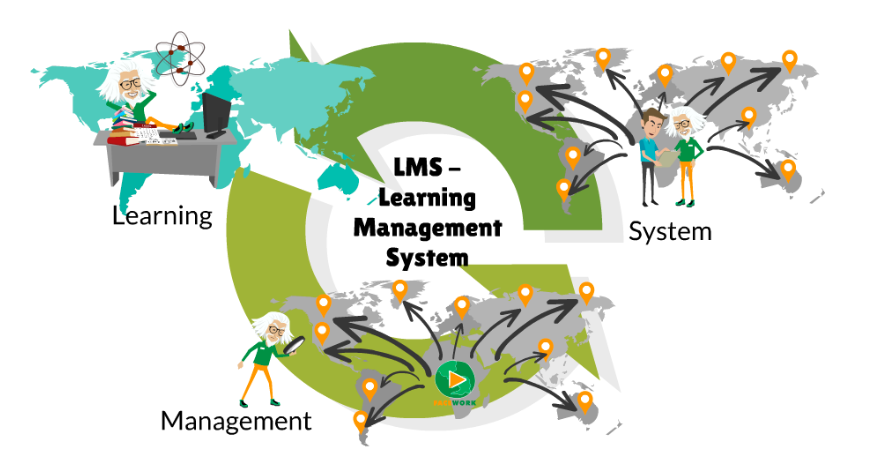
\includegraphics[scale=.5]{img/LMS}
		\end{center}
		\caption{Giới thiệu LMS}
		\label{refhinh1}
	\end{figure}
\end{center}
Learing Management System là tổ hợp gồm 3 từ riêng lẻ: Learning, Management và System. Ý nghĩa của 3 từ đó được giải thích như sau:
\begin{itemize}
	\item Ý nghĩa về Learning: Các chủ thể trong hệ thống học trực tuyến tạo ra các khóa học hay chương trình đào tạo, và muốn phân phối các sản giáo dục này đến những người sử dụng.
	\item Ý nghĩa về Management: Việc tạo ra các khóa học hay thay đổi, xóa bỏ là điều cần thiết. Bên cạnh đó, với Management, người dùng có thể sắp xếp, phân loại hay đánh giá các khóa học. Một cách đích thực, Management có nghĩa là sự quản lý các khóa học trực tuyến.
	\item Ý nghĩa về System: Như thông tin bên trên, LMS về cơ bản vẫn là một chương trình máy tính và là tập hợp của những công nghệ số, nên nhìn chung đây là một hệ thống, và người ta dùng hệ thống này để quản lý các khóa học/ chương trình đào tạo.
\end{itemize}
\subsection{Các thành tố cấu thành một LMS}
{Trên thế giới hiện tại có rất nhiều hệ thống LMS đến từ nhiều nhà cung cấp, nhưng cốt lõi, các hệ thống LMS này đều nhằm mục đích giải quyết các nhu cầu tương tác của các chủ thể chính trong hệ thống học trực tuyến, đó là người cung cấp nội dung học trực tuyến, người sử dụng nội dung học trực tuyến và người điều hành, quản lý tương tác học trực tuyến.}

{Theo cấu trúc, một LMS được cấu thành từ 2 thành phần chính:}
\begin{itemize}
	\item Thành phần công nghệ nền gồm các chức năng cốt lõi như tạo, quản lý và cung cấp các khóa học, chứng thực người dùng, cung cấp các dữ liệu hay thực hiện các thông báo,…Thành phần này được quản lý và điều khiển bởi người lập trình, người quản lý hệ thống.
	\item Thành phần thứ hai liên quan đến giao diện người dùng chạy trên nền các trình duyệt web (tương tự như Gmail/ Facebook). Thành phần này được dùng bởi các chủ thể trong hệ thống học trực tuyến như người quản lý, giảng viên và học viên.
\end{itemize}

{Theo chức năng, LMS là một tổ hợp gồm một số chức năng cốt lõi sau:}
\begin{itemize}
	\item Chức năng quản lý lưu trữ dữ liệu số: Chức năng này cho phép các chủ thể trên hệ thống E-Learning có thể đăng tải các khóa học cũng như các tài liệu số liên quan hỗ trợ người học. Các dữ liệu số được đăng tải có hệ thống phân loại theo định dạng tập tin, dung lượng, theo thời gian đăng tải,…và được kiểm soát nội dung.
	\item Chức năng bảo mật: Đây là chức năng rất quan trọng trong hệ thống LMS, nó bảo vệ hệ thống dữ liệu của các chủ thể một cách an toàn. Hơn thế nữa, các thông tin cá nhân liên quan các chủ thể hoặc các dữ liệu liên quan đến tài chính cũng được bảo vệ.
	\item Chức năng đáp ứng: 
	\begin{itemize}
		\item Tương thích đa chủng loại thiết bị truy cập: Chức năng này hỗ trợ nhiều thiết bị công nghệ truy cập hệ thống LMS như máy tính bàn, laptop, thiết bị di động, hay máy tính bảng,...
		\item Băng thông đảm bảo lưu lượng người dùng truy cập vào hệ thống học trực tuyến.
	\end{itemize}
	\item Chức năng đa chủ thể: Tính năng này hỗ trợ một lớp học/ một chương trình đào tạo trực tuyến có sự tham gia tương tác cùng lúc bởi nhiều giáo viên và nhiều học viên, họ đến từ nhiều nơi trên toàn thế giới.
	\item Chức năng đa ngôn ngữ: Một LMS dùng làm mục đích kinh doanh, vận hành trên môi trường Internet có thể tiếp cận một cá nhân bất kỳ tại một quốc gia nào đó trên thế giới. Cho nên, việc cho phép chuyển đổi các ngôn ngữ qua lại hoặc ít nhất là một ngôn ngữ quốc tế cần được tích hợp vào hệ thống LMS.
	\item Kiểm soát đăng ký: Khả năng kiểm soát và tùy chỉnh quá trình đăng ký học trực tuyến.
	\item Lịch: Chức năng này thiết lập lịch cho các chương trình học tập trực tuyến như lịch học, thời hạn khóa học, lịch thi,...
	\item Chức năng quản lý giao dịch: Chức năng này cho phép hệ thống LMS kiểm soát được các giao dịch phát sinh khi tương tác với các khóa học trực tuyến của các chủ thể: giao dịch giữa học viên với người cung cấp dịch vụ E-Learning (học phí); Giao dịch giữa người cung cấp dịch vụ E-Learning với tác giả khóa học (thù lao giảng viên/ tiền phân chia lợi nhuận khóa học) hay các giao dịch tiền ký gửi học theo hình thức ví điện tử,...
	\item Chức năng quản lý tương tác, hỗ trợ:
	\begin{itemize}
		\item Tương tác giữa các học viên: Chức năng này cho phép các học viên có thể trao đổi thông tin, trao đổi tài liệu qua hệ thống chat, email hoặc SMS,... nhằm tương tác hỗ trợ học tập.
		\item Tương tác giữa học viên với tác giả: Chức năng cho phép giữa học viên và tác giả khóa học/ chương trình đào tạo có thể trao đổi thông tin hoặc đánh giá, nhận xét lẫn nhau.
		\item Tương tác giữa học viên, giảng viên với quản trị hệ thống: Chức năng cho phép 2 chủ thể là người cung cấp kiến thức khóa học và người nhận khóa học tương tác trao đổi với quản trị hệ thống. Các vấn đề tương tác liên quan như các quy định, chế độ,...
	\end{itemize}
	\item Chức năng thi, kiểm tra: Chức năng này cho phép các học viên tham gia kiểm tra năng lực học tập hoặc xếp loại sau khai trải qua quá trình học. Các hình thức thi và kiểm tra phổ biến trên hệ thống LMS như trắc nghiệm, nhiệm vụ tương tác thông qua game,...
	\item Chức năng theo dõi, kiểm soát: Chức năng này cho phép người học hoặc chủ thể trung gian quản lý người học có thể kiểm soát tiến trình học tập cũng như năng lực người học qua từng giai đoạn.
\end{itemize}
\subsection{Ưu điểm của LMS}
Từ khi xuất hiện lần đầu được dùng để mô tả một phần hệ thống quản lý của hệ thống học tập PLATO K-12, LMS đã dần phát triển ngày càng đa dạng tương ứng với nhiều mô hình giáo dục khác nhau trên toàn thế giới. Cho dù phân hóa theo đặc thù của từng đơn vị áp dụng, song, hệ thống LMS nói chung vẫn luôn trên mình như là một bản chất các ưu điểm:
\begin{itemize}
	\item Dễ dàng thích nghi và tái sử dụng theo thời gian.
	\item Có nhiều sự lựa chọn cho từng đối tượng tạo lập ra các chương trình giảng dạy như phương thức học tập, phương thức thanh toán, các hình thức tương tác, kiểm tra đánh giá,...
	\item Có thể dễ dàng tiếp cận các sản phẩm giáo dục của bên thứ 3 qua đó làm giảm chi phí sản xuất cho doanh nghiệp.
	\item Các doanh nghiệp có thể tận dụng LMS như là một công cụ để nhân viên tự đánh giá, kiểm tra qua đó rèn luyện nâng cao năng lực chuyên môn. Và với LMS, doanh nghiệp vừa tiết kiệm chi phí đào tạo vừa nhận được nhiều hơn các giá trị đến từ nhân viên.
\end{itemize}

\section{Tại sao chọn Moodle?}
\subsection{Giới thiệu về Moodle \cite{aboutmoodle}}
{Moodle (viết tắt của Modular Object-Oriented Dynamic Learning Environment) được sáng lập năm 1999 bởi Martin Dougiamas với mục đích tạo ra những khóa học trực tuyến có sự tương tác cao. Tính mã mở cùng sự linh hoạt của Moodle giúp người phát triển có khả năng thêm vào các module cần thiết một cách dễ dàng. Đây là phần quan trọng của hệ thống E-learning trong hỗ trợ học trực tuyến. Moodle được đánh giá là một thiết kế hướng tới giáo dục, dành cho những người làm trong giáo dục. Với giao diện trực quan dễ sử dụng, giáo viên chỉ mất một thời gian ngắn để làm quen và có thể sử dụng thành thạo. Moodle phù hợp với nhiều cấp học và hình thức đào tạo: phổ thông, đại học, cao đẳng, không chính quy hay trong các tổ chức, công ty.}


{Thông qua số liệu tháng 1 năm 2019 \cite{moodlestats} ta có được kết quả sau:}
\begin{center}
	\begin{table}[!htp]
		\centering
		\begin{tabular}{|l|r|}
			\hline 
			Trang web đã đăng ký & 107,517 \\ 
			\hline 
			Quốc gia đã đăng ký & 228 \\ 
			\hline 
			Khóa học đã đăng ký & 18,357,666 \\ 
			\hline 
			Lượng người dùng & 150,625,167 \\ 
			\hline 
		\end{tabular} 
		\caption{Thống kê Moodle}
		\label{bang1}
	\end{table}
\end{center}
\begin{center}
	\begin{table}[!htp]
		\centering
		\begin{tabular}{|l|r|}
			\hline 
			{\bf Quốc gia} & {\bf Số lượng người dùng} \\ 
			\hline 
			Mỹ & 9,971 \\ 
			\hline 
			Tây Ban Nha & 8,470 \\ 
			\hline 
			Mê Hi Cô & 5,287 \\ 
			\hline 
			Bra-xin & 5,260 \\ 
			\hline 
			Đức & 3,563 \\ 
			\hline 
			Anh & 3,458 \\ 
			\hline 
			Nga & 2,949 \\ 
			\hline 
			Ý & 2,923 \\ 
			\hline 
			Colombia & 2,498 \\ 
			\hline 
			Pháp & 2,464 \\ 
			\hline 
		\end{tabular} 
		\caption{Top 10 quốc gia đăng ký Moodle}
		\label{bang3}
	\end{table}
\end{center}

Từ kết quả trên ta có thể thấy được mức độ thông dụng của Moodle trong việc tạo ra một hệ thống quản lý học tập trực tuyến.
\subsection{Các chức năng cơ bản của Moodle \cite{featuremoodle}}
\begin{itemize}
	\item {\bf Trò chuyện:} Mô-đun trò chuyện cho phép người dùng có thể trao đổi thông tin theo thời gian thực. Đây quả thực là một cách hiệu quả để chúng ta có thể chia sẻ những sự hiểu biết cũng như những ý kiến cá nhân về chủ đề đang được thảo luận. Bên cạnh đó, mô-đun trò chuyện cũng chứa thêm những tính năng để quản lý cuộc trò chuyện một cách chủ động hơn.
	\item {\bf Cơ sở dữ liệu:} Mô-đun cơ sở dữ liệu cho phép giảng viên và sinh viên có thể hiện thị và tìm kiếm các mục trong một chủ đề, các mục này có thể là hình ảnh, tập tin, đường dẫn,... Tính năng đặc biệt của mô-đun cơ sở dữ liệu đó là chúng ta có thể tự thiết lập cơ sở dữ liệu để quyết định số lượng mục tối thiểu, tối đa mà một người dùng được phép tương tác,...
	\item {\bf Diễn đàn:} Diễn đàn là nơi để giảng viên, sinh viên cùng nhau thảo luận về nội dung bài học. Bằng việc đăng ký tham gia một diễn đàn, người tham gia sẽ nhận được thông tin những bài đăng mới nhất thông qua email. Giảng viên có thể thêm tất cả mọi người vào diễn đàn của mình nếu họ muốn vì thế giảng viên có thể liên hệ được với tất cả sinh viên trong khóa học của mình. Tất cả các khóa học của Moodle đi kèm theo là một diễn đàn Tin tức không thể xóa, tuy nhiên người dùng vẫn có thể thêm một diễn đàn mới.
	\item {\bf Bảng câu hỏi:} Mô-đun bảng câu hỏi cho phép giảng viên tạo ra một bản khảo sát hoặc bản câu hỏi để sinh viên điền vào nhằm đánh giá sự hài lòng của bạn về khóa học. Đặc biệt mô-đun này có tính năng ẩn danh người tham gia điền khảo sát giúp cho sinh viên thoải mái nêu lên những suy nghĩ của mình.
	\item {\bf Lịch biểu:} Mô-đun này cho phép giảng viên tạo ra những lịch biểu và yêu cầu sinh viên đăng ký vào những thời gian phù hợp với mình. Điều này là rất cần thiết cho các cuộc họp giữa sinh viên và giáo viên.
	\item {\bf Bài giảng:} Cho phép giảng viên tạo ra lộ trình bài học thông qua tài liệu. Nó gồm nhiều phần, mỗi phần thường kết thúc bằng một câu hỏi và một số câu trả lời có thể có. Tùy vào sự lựa chọn của học viên, nếu đúng họ sẽ được chuyển sang phần kế tiếp, còn nếu sai họ sẽ được đưa trở lại trang trước. Đây là một công cụ hữu ích để sinh viên học tập, nghiên cứu.
	\item {\bf Bài tập:} Mô-đun này cho phép sinh viên nộp bài một cách trực tuyến, bài tải lên có thể ở bất kỳ loại tệp nào (Word, Powerpoint, Zip, Video,...). Giảng viên có thể chấm điểm dựa vào đó và đưa ra phản hồi.
	\item {\bf Bài kiểm tra:} Mô-đun bài kiểm tra cho phép giáo viên thiết kế các bài kiểm tra bao gồm nhiều câu hỏi. Đây là một công cụ rất tiện lợi cho các giảng viên. Thật vậy bài kiểm tra điện tử có thể làm nhiều việc mà bài kiểm tra truyền thống trên giấy không thể. Người dùng có thể tạo ra các loại câu hỏi khác nhau, mở ngẫu nhiên câu hỏi có trong ngân hàng câu hỏi, cho phép học viên làm lại câu hỏi nhiều lần và có tính năng chấm điểm ngay khi học viên kết thúc bài kiểm tra.
	\item {\bf Scorm:} Moodle có mô-đun cho cả hai định dạng là SCORM hoặc AICC cho phép bạn dễ dàng đóng gói, tái sử dụng nội dung đào tạo của mình hoặc từ một khóa học khác.
	\item {\bf Khảo sát:} Các cuộc khảo sát được tạo ra nhằm mục đích thu thập thông tin về mức độ hài lòng của người học đối với khóa học. 
	
\end{itemize}

\subsection{Nguyên nhân lựa chọn Moodle}
Tầm quan trọng của Moodle được thể hiện tốt trong nhiều báo cáo, được cộng đồng chấp nhận và có nhiều khóa học hiện nay trên hầu hết nhiều quốc gia đang hoạt động dựa trên nền tảng Moodle. Nó cung cấp cho người dùng nhiều tính năng hữu ích như đăng tin tức, bài tập, bài giảng, video,... Điểm mạnh nhất của Moodle là có một cộng đồng phát triển to lớn, các diễn đàn thảo luận về những tích cực, chia sẻ mẹo, mã nguồn giúp cho những người dùng mới dễ dàng tiếp cận hơn.

Để thấy rõ hơn vì sao chúng em lựa chọn Moodle để nghiên cứu và xây dựng công cụ hỗ trợ các khóa học trực tuyến. Theo tìm hiểu chúng em đưa ra những lý do sau: \cite{whymoodle}
\begin{itemize}
	\item Moodle là một OSS, nghĩa là người dùng có thể tải Moodle miễn phí, sử dụng và chỉnh sửa nó một cách cá nhân, thậm chí chúng ta cũng có thể phân phối nó theo các điều khoản của giấy phép GNU.
	\item Nó là một nơi để giáo viên có thể chia sẻ những tài liệu, giao bài tập, trao đổi,... với học viên của mình để việc học trở nên dễ dàng hơn.
	\item Moodle có thể sử dụng hầu hết các server viết bằng PHP, chúng ta có thể dễ dàng sử dụng và nâng cấp nó bằng ngôn ngữ PHP.
	\item Điểm đặc biệt của Moodle là sự kết hợp giữa việc dạy học với công nghệ, bên cạnh đó điểm mạnh của Moodle so với các hệ thống khác chính là nền tảng vững chắc của nó trong việc xây dựng một khóa học trực tuyến.
	\item Moodle được sử dụng trên nhiều quốc gia trên thế giới như số liệu bảng 2.1 chúng ta có thể thấy Moodle mạnh mẽ như thế nào.
	\item Moodle chạy được trên tất cả hệ điều hành thông dụng ngày nay như Windows, Linux, Unix. Nó được xây dựng bằng ngôn ngữ PHP, sử dụng MySQL, Oracle làm cơ sở dữ liệu.
	\item Moodle rất dễ dùng với giao diện trực quan, giáo viên chỉ cần một thời gian ngắn để làm quen và có thể sử dụng thành thạo Moodle. Do giao diện thiết kế sử dụng đơn giản nên giáo viên có thể tự cài và nâng cấp Moodle.
	\item Moodle thì rất tốt trong việc tạo điều kiện cho các sinh viên khoa học máy tính (công nghệ thông tin) có cơ hội để phát triển một module cho LMS Moodle. Sinh viên có thể xây dựng các module cho LMS Moodle và chia sẻ nó cho cộng đồng toàn cầu. 
	\item Tài liệu hỗ trợ của Moodle rất đồ sộ và chi tiết.
	\item Tuy là phần mềm mã nguồn mở, như chất lượng của Moodle rất tốt, chất lượng bằng hoặc tốt hơn Blackboard /WebCT trong nhiều khía cạnh. Bởi cộng đồng các nhà giáo dục, chuyên gia máy tính, và các chuyên gia thiết kế giảng dạy chính là những người phát triển Moodle, và kết quả là bạn có trong tay một sản phẩm đáp ứng tốt các yêu cầu người dùng.
	\item Bảng so sánh chức năng với các hệ thống khác cũng sẽ làm ta thấy rõ điều này (so sánh với các hệ thống thương mại (không phải mã nguồn mở) Blackboard và WebCT): \cite{moodle-blackboard-webct}
	\begin{center}
		\begin{table}[!htp]
			\centering
			\begin{tabular}{|c|c|c|c|}
				\hline 
				{\bf Tính năng} & {\bf Blackboard} & {\bf WebCT} & {\bf Moodle} \\ 
				\hline 
				Upload và chia sẻ tài liệu & Có & Có & Có \\ 
				\hline 
				Tạo một trang web và soạn thảo với HTML online & Không & Có & Có \\ 
				\hline 
				Thảo luận online & Có & Có & Có \\ 
				\hline 
				Đánh giá học viên & Không & Có & Có \\ 
				\hline 
				Chat Online & Có & Có & Có \\ 
				\hline 
				Xem các thông tin của học viên khác & Không & Không & Có \\ 
				\hline 
				Khảo sát và điều tra & Có & Có & Có \\ 
				\hline 
				Bảng xếp hạng & Có & Có & Có \\ 
				\hline 
				Học viên tự đánh giá bài làm của mình & Không & Không & Có \\ 
				\hline 
				Nhóm học viên & Có & Có & Có \\ 
				\hline 
				Nhật ký học viên & Không & Không & Có \\ 
				\hline 
				Đánh dấu thuật ngữ & Không & Không & Có \\ 
				\hline 
			\end{tabular} 
			\caption{Bảng so sánh Moodle, Blackboard và WebCT}
			\label{bang2}
		\end{table}
	\end{center}
	Thông qua bảng trên ta có thể thấy được tất cả các so sánh đều chỉ ra rằng Moodle là ưu việt nhất cho e-learning.
\end{itemize}

\subsection{Sự hạn chế của Moodle}
Bên cạnh những lợi ích mà Moodle mang lại thì chúng ta không thể không kể đến những mặt hạn chế của Moodle như sau:

\begin{itemize}
	\item Moodle thường chỉ dành cho lập trình viên. Nó trở nên rất phức tạp đối với người dùng bình thường. Thật vậy có hơn 66\% trong số người dùng là giáo viên, nhà nghiên cứu và quản trị viên. \cite{limitmoodle:1}
	\item Lập trình viên mới bắt đầu sẽ khó để cài đặt Moodle, vì có nhiều từ ngữ chuyên ngành kỹ thuật trong hướng dẫn cài đặt. \cite{limitmoodle:2}
	\item Moodle sẽ không hoạt động nếu như không có quản trị viên làm việc được với cả giáo viên và kỹ thuật viên để tạo ra tài nguyên trực tuyến. \cite{whymoodle}
	\item Mặc dù tài liệu tham khảo về Moodle rất nhiều nhưng hầu hết đều được viết bằng tiếng anh nên không phải ai cũng dễ dàng tiếp cận.
\end{itemize}

\section{Block(khối) trong Moodle}
\subsection{Khối là gì?}
Một khối thể hiện thông tin trong một khu vực nhỏ trong các cột bên. Trong ví dụ, khối hiển thị lịch, tin tức mới nhất hoặc là tên học viên đã ghi danh vào khóa học.

Block là các công cụ nằm ở cột bên trái và phải. Có nhiều Block được cung cấp sẵn cho bạn. Một số khối phổ biến là: People, Navigation, Settings, Search Forum, Campus Links and Calendar. Bạn có thể tạo một khóa học tùy ý bao gồm các khối liên quan đến khóa học của bạn. \cite{blockmoodle}

Các gói tiêu chuẩn có sẵn khi bạn cài đặt một Moodle. Bạn cũng có thể cài đặt thêm các khối có sẵn thông qua http://moodle.org/

Ở trang quản trị của Moodle, ta có thể thay đổi vị trí của các khối (khu vực quản trị, khu vực điều hướng, calendar…). Ta cũng có thể thêm các khối mới hoặc ẩn đi các khối đang hiển thị. Thậm chí ta có thể thiết lập các quyền cho các nhóm người dùng có thể thấy hoặc không thấy khối khi họ đăng nhập vào tài khoản của mình.

Tại khu vực quản trị, ta chọn Cài đặt trang ngoài \ Bật chế độ chỉnh sửa. Sau khi bật chế độ chỉnh sửa thì trên mỗi khối sẽ xuất hiện các button để cho ta thao tác.
\begin{center}
	\begin{figure}[htp]
		\begin{center}
			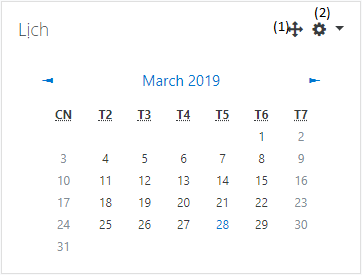
\includegraphics[scale=1]{img/lich}
		\end{center}
		\caption{Khối lịch trong Moodle}
		\label{refhinh2}
	\end{figure}
\end{center}
- Button (1) cho ta có thể dễ dàng kéo thả khối đến những vị trí khác trên giao diện.\\
- Button (2) cho phép ta thực hiện các thao tác như ẩn khối, xóa khối khỏi giao diện, thiết lập các nhóm người dùng có thể thấy hoặc không thấy khối.

Ta cũng có thể thêm một khối mới vào giao diện. Bằng cách lựa chọn khối mà ta muốn thêm trong mục "Thêm Khối".
\begin{center}
	\begin{figure}[htp]
		\begin{center}
			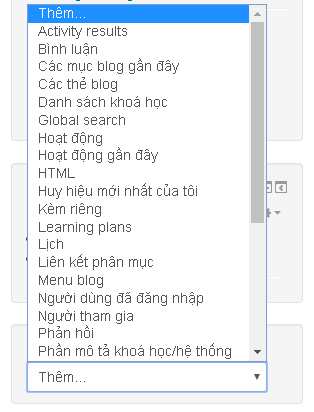
\includegraphics[scale=0.8]{img/addblock}
		\end{center}
		\caption{Giao diện lựa chọn block ta muốn thêm}
		\label{refhinh3}
	\end{figure}
\end{center}

\vskip 4cm
Giao diện sau khi thêm khối:
\begin{center}
	\begin{figure}[htp]
		\begin{center}
			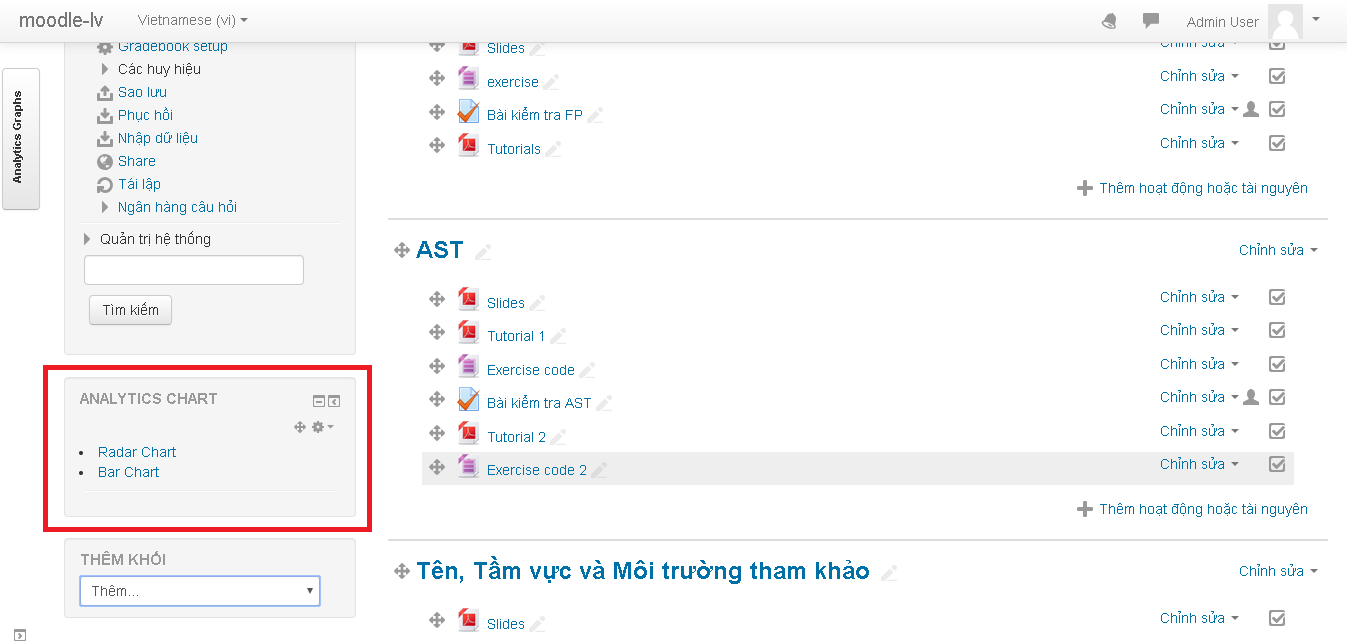
\includegraphics[scale=0.5]{img/block}
		\end{center}
		\caption{Khối đã được thêm vào}
		\label{refhinh4}
	\end{figure}
\end{center}

\subsection{Một số ví dụ về khối}
\subsubsection{Khối điều hướng:}
Khối điều hướng xuất hiện trong mỗi trang của trang web. Nó chưa một Menu cây mở rộng bao gồm: Trang chủ, các trang của hệ thống, hồ sơ và khóa học. Những gì xuất hiện trong khối điều hướng phụ thuộc vào vai trò của người dùng và họ đang ở đâu trong trang Moodle.
\begin{center}
	\begin{figure}[htp]
		\begin{center}
			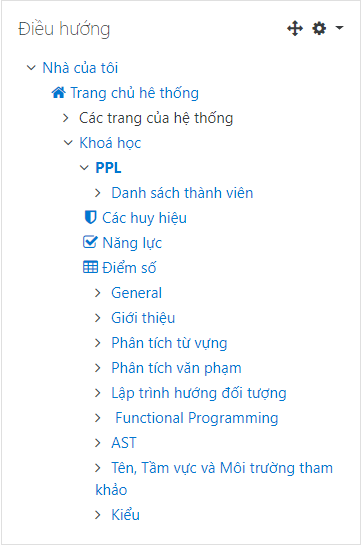
\includegraphics[scale=0.6]{img/khoidieuhuong}
		\end{center}
		\caption{Khối điều hướng}
		\label{refhinh5}
	\end{figure}
\end{center}

\subsubsection{Khối cài đặt:}
Khối cài đặt cung cấp các liên kết đến các trang cài đặt. Các mục Menu chính (Quản tri khóa học và hồ sơ của tôi) chứa nột Menu con và có thể được thu gọn hoặc mở rộng để hiển thị Menu như hình bên dưới.
\begin{center}
	\begin{figure}[htp]
		\begin{center}
			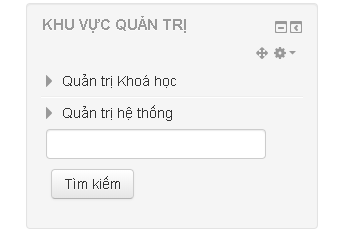
\includegraphics[scale=1]{img/khoicaidat}
		\end{center}
		\caption{Khối cài đặt}
		\label{refhinh6}
	\end{figure}
\end{center}

\subsubsection{Khối điều hướng bài kiểm tra:}
Khối điều hướng bài kiểm tra nằm ở góc trên bên phải. Bạn có thể sử dụng nó để di chuyển đến bất kì câu hỏi. Các hộp câu hỏi cho trang hiện tại được in đậm. Các câu hỏi được gắn cờ sẽ có “góc đỏ” trong hộp của câu hỏi.
\begin{center}
	\begin{figure}[htp]
		\begin{center}
			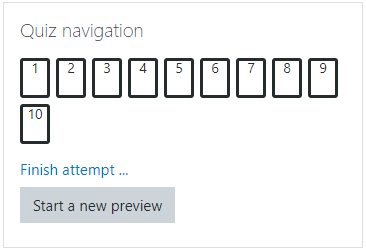
\includegraphics[scale=1]{img/khoibaikiemtra}
		\end{center}
		\caption{Khối điều hướng bài kiểm tra}
		\label{refhinh7}
	\end{figure}
\end{center}

\section{Tổng quan về ChartJS}
\subsection{ChartJS là gì? \cite{chartjs:1}}
ChartJS là một trong những dự án mã nguồn mở giúp cho mọi người có thể vẽ những biểu đồ thể hiện số liệu trên website một cách dễ dàng và đẹp nhất. Tính đến tháng 1 năm 2019 dự án này hiện có đến 41.000 stars và 2600 lượt commit trên Github và được cập nhật thường xuyên. Những ưu điểm nổi bật nhất của ChartJS là:
\begin{itemize}
	\item Dự án mã nguồn mở: cả cộng đồng phát triển và khắc phục lỗi.
	\item Tương thích tốt với HTML.
	\item Hơn 8 kiểu biểu đồ phổ biến nhất hiện nay.
	\item Có hỗ trợ responsive giúp hiển thị đẹp nhất trên tất cả các thiết bị từ Desktop, Tablet, Mobile.
\end{itemize}

\subsection{Cách cài đặt ChartJS \cite{chartjs:2}}
Có nhiều cách để cài đặt thư viện ChartJS nhưng chúng em xin đề cập những cách cài đặt phổ biến thông qua những công cụ sau:
\begin{itemize}
	\item npm: npm install chart.js --save
	\item Bower: bower install chart.js --save
	\item CDN: Truy cập link https://cdnjs.com/libraries/Chart.js
	\item Github: Truy cập link sau để tải về bản mới nhất https://github.com/chartjs/Chart.js/releases
\end{itemize}

\subsection{Sử dụng ChartJS trên web}
Để sử dụng ChartJS chúng ta cần thực hiện theo các bước sau: \cite{chartjs:3}
\begin{itemize}
	\item Khai báo thư viện ChartJS và Bootstrap.
	\item Tạo thẻ <canvas> trong trang web
	\begin{center}
		\begin{figure}[htp]
			\begin{center}
				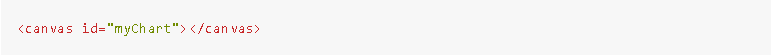
\includegraphics[scale=1]{img/canvas}
			\end{center}
			\caption{Thẻ canvas}
			\label{refhinh8}
		\end{figure}
	\end{center}
	\item Sử dụng Javascript để đăng ký biểu đồ.
	\begin{center}
		\begin{figure}[htp]
			\begin{center}
				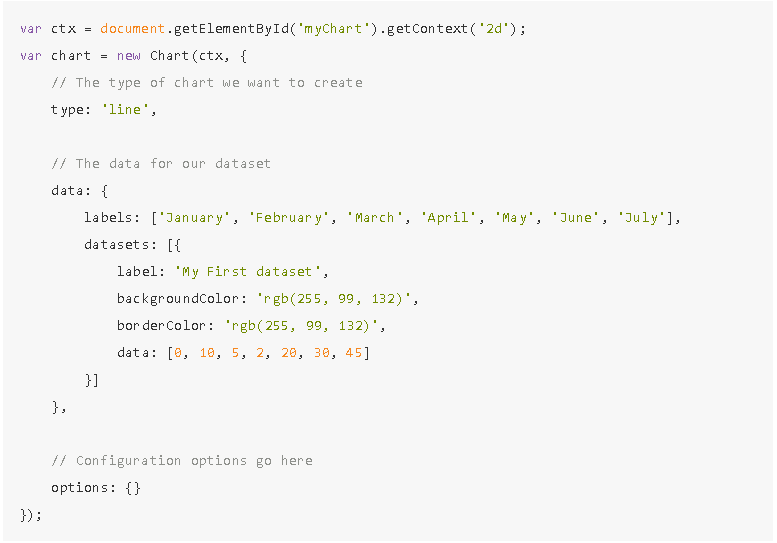
\includegraphics[scale=1]{img/chartjs}
			\end{center}
			\caption{Tạo một biểu đồ thông qua Javascript}
			\label{refhinh9}
		\end{figure}
	\end{center}
\end{itemize}
	
	\newpage
	\setcounter{chapter}{2}
\fontsize{13}{5}\selectfont
\chapter{Phân tích hệ thống}
EHAT sẽ sử dụng các bảng có sẵn trong database của hệ thống học tập Moodle để lấy thông tin, phân tích và sẽ trả về những kết quả mà ta mong đợi. Chính vì thế nhóm chúng em sẽ nêu ra những use case cũng như những database của Moodle cần thiết phục vụ cho quá trình xây dựng công cụ EHAT.
\section{Nghiên cứu use case của hệ thống Moodle}
\subsection{Những hành động cơ bản của giáo viên và học sinh có sẵn trên Moodle}
Khi chưa thêm công cụ EHAT giáo viên và học sinh có những hành động cơ bản sau: \cite{usecase:1}
\begin{itemize}
	\item Đối với giáo viên
	\begin{center}
		\begin{figure}[htp]
			\begin{center}
				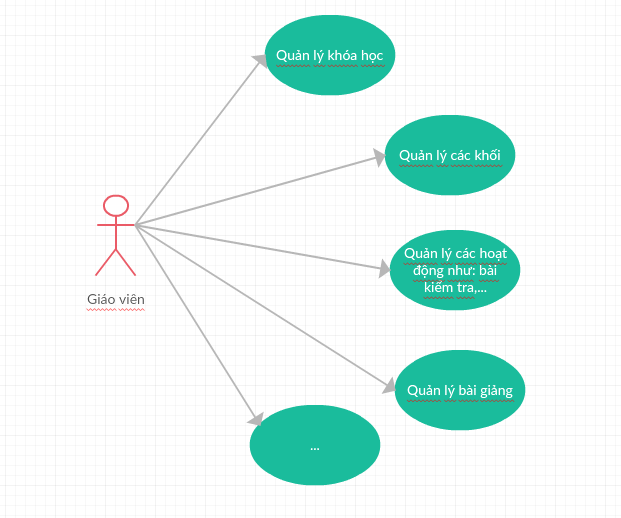
\includegraphics[scale=0.7]{img/usecasegv}
			\end{center}
			\caption{Use case thể hiện hành động cơ bản của GV}
			\label{refhinh10}
		\end{figure}
	\end{center}
	\vskip 1cm 
	\item Đối với học sinh, sinh viên
	\begin{center}
		\begin{figure}[htp]
			\begin{center}
				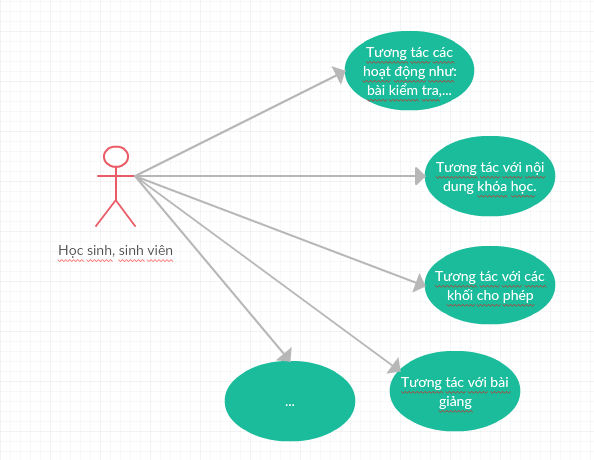
\includegraphics[scale=0.7]{img/usecasehs}
			\end{center}
			\caption{Use case thể hiện hành động cơ bản của HS, SV}
			\label{refhinh11}
		\end{figure}
	\end{center}
\end{itemize}

\subsection{Những hành động khi thêm công cụ EHAT}
Sau khi thêm vào hệ thống công cụ EHAT:
\begin{itemize}
	\item Đối với giáo viên
	\begin{center}
		\begin{figure}[htp]
			\begin{center}
				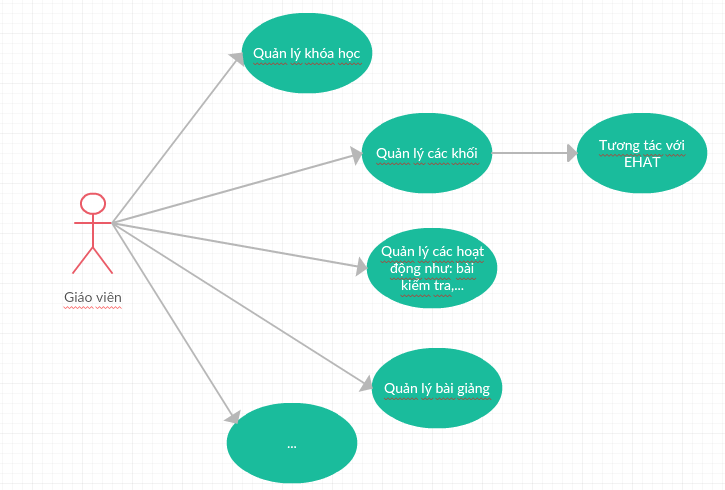
\includegraphics[scale=0.65]{img/usecasegvehat}
			\end{center}
			\caption{Use case thể hiện hành động cơ bản của GV khi có EHAT}
			\label{refhinh12}
		\end{figure}
	\end{center}
	\vskip 3cm
	\item Đối với học sinh, sinh viên
	\begin{center}
		\begin{figure}[htp]
			\begin{center}
				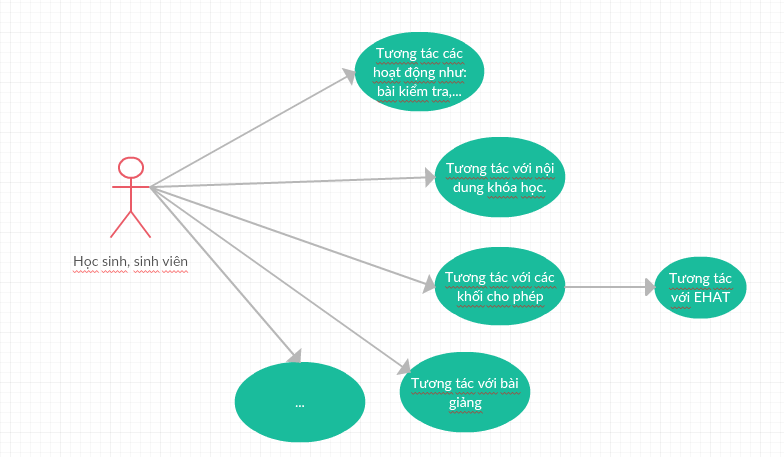
\includegraphics[scale=0.7]{img/usecasehsehat}
			\end{center}
			\caption{Use case thể hiện hành động cơ bản của HS, SV khi có EHAT}
			\label{refhinh13}
		\end{figure}
	\end{center}
\end{itemize}

Chi tiết các hoạt đông mà EHAT mang lại:
\begin{itemize}
	\item Đối với giáo viên
	\begin{center}
		\begin{figure}[htp]
			\begin{center}
				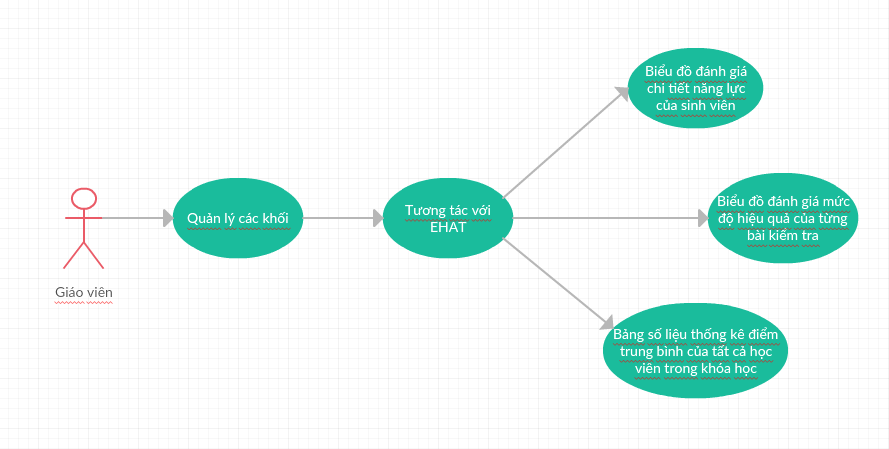
\includegraphics[scale=0.7]{img/chitietehatgv}
			\end{center}
			\caption{Các hoạt động EHAT mang lại cho GV}
			\label{refhinh14}
		\end{figure}
	\end{center}
	\vskip 4cm
	\item Đối với học sinh, sinh viên
	\begin{center}
		\begin{figure}[htp]
			\begin{center}
				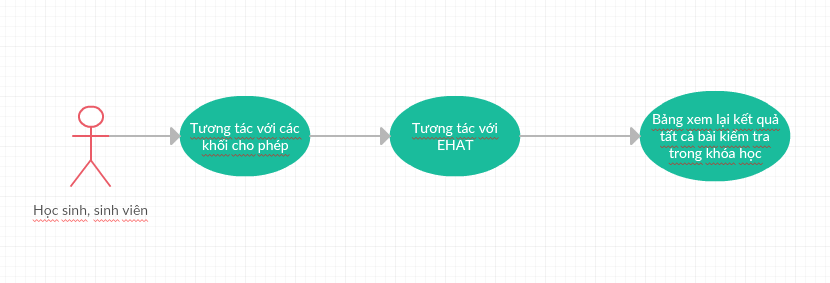
\includegraphics[scale=0.7]{img/chitietehaths}
			\end{center}
			\caption{Các hoạt động EHAT mang lại cho HS, SV}
			\label{refhinh15}
		\end{figure}
	\end{center}
\end{itemize}

\newpage
\section{Database của Moodle}

\begin{center}
	\begin{figure}[htp]
		\begin{center}
			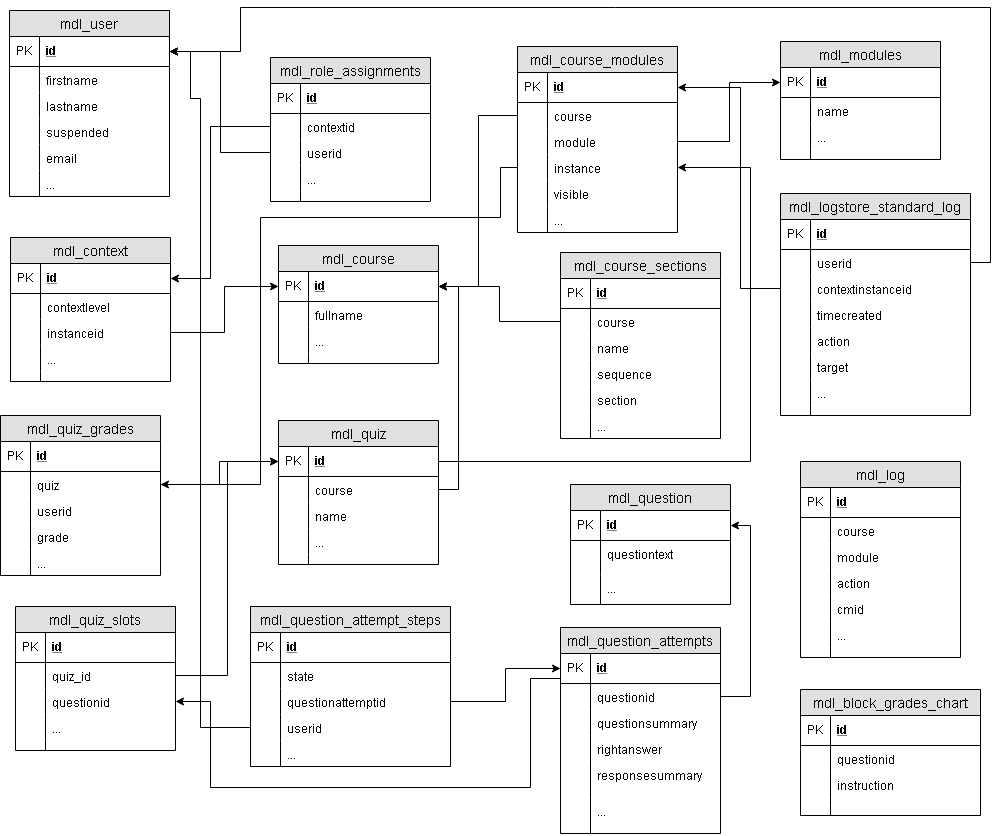
\includegraphics[scale=0.5]{img/database}
		\end{center}
		\caption{Các bảng được sử dụng}
		\label{refhinh19}
	\end{figure}
\end{center}

\newpage
Chi tiết cấu trúc cơ bản được sử dụng của từng bảng trên:
\begin{itemize}
	\item Bảng mdl\_user
	\begin{center}
		\begin{table}[!htp]
			\centering
			\begin{tabular}{|c|c|}
				\hline 
				id & Id người dùng \\ 
				\hline 
				auth &  \\ 
				\hline 
				confirmed & Kiểm tra người dùng đã được xác nhận chưa (1 hoặc 0) \\ 
				\hline 
				deleted & Xóa người dùng (1 hoặc 0) \\ 
				\hline 
				username & Tài khoản \\ 
				\hline 
				password & Mật khẩu \\ 
				\hline 
				idnumber &  \\ 
				\hline 
				firstname & Họ và lót người dùng \\ 
				\hline 
				lastname & Tên người dùng \\ 
				\hline 
				email & Email người dùng \\ 
				\hline 
				emailstop & Mặc định 0 \\ 
				\hline 
				phone1 & Số điện thoại thứ 1 \\ 
				\hline 
				phone2 & Số điện thoại thứ 2 \\
				\hline 
				address & Địa chỉ người dùng \\ 
				\hline 
				city & Thành phố \\ 
				\hline 
				country & Quốc gia \\ 
				\hline 
				lang & Ngôn ngữ \\
				\hline 
				timezone & Múi giờ \\ 
				\hline 
				firstaccess & Ngày truy cập đầu tiên \\ 
				\hline 
				lastaccess & Ngày truy cập cuối cùng \\ 
				\hline 
				lastlogin & Ngày đăng nhặp đầu tiên \\ 
				\hline 
				currentlogin & Thời gian người dùng đăng nhập hiện tại \\ 
				\hline 
				lastip & Thiết bị đăng nhập cuối cùng \\ 
				\hline 
				secret & Câu hỏi bảo mật \\ 
				\hline 
				picture & Ảnh đại diện \\
				\hline 
				description & Mô tả thông tin người dùng \\ 
				\hline 
				descriptionformat &  \\ 
				\hline 
				mailformat & HTML hoặc plaintext \\
				\hline 
				timecreated & Ngày đăng ký \\ 
				\hline 
				timemodified & Ngày chỉnh sửa \\
				\hline 
				... & ... \\
				\hline
			\end{tabular}
			\caption{Chi tiết bảng mdl\_users}
			\label{bang4}
		\end{table}
	\end{center}
	\newpage
	\item Bảng mdl\_role\_assignments
	\begin{center}
		\begin{table}[!htp]
			\centering
			\begin{tabular}{|c|c|}
				\hline 
				id & Khóa chính của bảng \\ 
				\hline 
				roleid & Khóa ngoại đến bảng role(Nơi lưu vai trò người dùng) \\ 
				\hline 
				contextid & Khóa ngoại đến bảng context \\ 
				\hline 
				userid & Id của người dùng \\ 
				\hline 
				timemodified & Thời gian chỉnh sửa bảng \\ 
				\hline 
				modifierid & Người chỉnh sửa \\ 
				\hline 
				... & ... \\
				\hline
			\end{tabular} 
			\caption{Chi tiết bảng mdl\_role\_assignments}
			\label{bang5}
		\end{table}
	\end{center}
	\item Bảng mdl\_context
	\begin{center}
		\begin{table}[!htp]
			\centering
			\begin{tabular}{|c|c|}
				\hline 
				id & Khóa chính của bảng \\ 
				\hline 
				contextlevel & Mức độ của một phạm vi trong moodle(50 là khóa học, 70 là câu hỏi,...) \\ 
				\hline 
				instanceid & Tùy thuộc vào contextlevel mà instanceid sẽ tham khảo đến \\ & id của phạm vi tương ứng \\ 
				\hline 
				... & ... \\
				\hline
			\end{tabular} 
			\caption{Chi tiết bảng mdl\_context}
			\label{bang6}
		\end{table}
	\end{center}
	\item Bảng mdl\_course
	\begin{center}
		\begin{table}[!htp]
			\centering
			\begin{tabular}{|c|c|}
				\hline 
				id & Id khóa học \\ 
				\hline 
				category &  \\ 
				\hline 
				sortorder &  \\ 
				\hline 
				fullname & Tên đầy đủ của khóa học \\ 
				\hline 
				shortname & Tên viết tắt khóa học \\ 
				\hline 
				... & ... \\
				\hline
			\end{tabular} 
			\caption{Chi tiết bảng mdl\_course}
			\label{bang7}
		\end{table}
	\end{center}
	\newpage
	\item Bảng mdl\_course\_modules
	\begin{center}
		\begin{table}[!htp]
			\centering
			\begin{tabular}{|c|c|}
				\hline 
				id & Khóa chính của bảng \\ 
				\hline 
				course & Tham khảo đến khóa học tương ứng \\ 
				\hline 
				module & Tham khảo đến mô-đun tương ứng trong Moodle \\ 
				\hline 
				instance & Tùy thuộc vào module mà instance sẽ tham khảo đến \\ & id của phạm vi tương ứng \\  
				\hline 
				visible & Điều kiện để thấy mô-đun(1: thấy, 0: ẩn) \\  
				\hline 
				... & ... \\ 
				\hline 
			\end{tabular}
			\caption{Chi tiết bảng mdl\_course\_modules}
			\label{bang8}
		\end{table}
	\end{center}
	\item Bảng mdl\_course\_sections
	\begin{center}
		\begin{table}[!htp]
			\centering
			\begin{tabular}{|c|c|}
				\hline 
				id & Khóa chính \\ 
				\hline 
				course & Liên kết đến khóa học \\ 
				\hline 
				section &  \\ 
				\hline 
				sequence & Chuỗi những mô-đun của khóa học \\ 
				\hline 
				... & ... \\ 
				\hline 
			\end{tabular} 
			\caption{Chi tiết bảng mdl\_course\_sections}
			\label{bang9}
		\end{table}
	\end{center}
	\item Bảng mdl\_quiz\_grades
	\begin{center}
		\begin{table}[!htp]
			\centering
			\begin{tabular}{|c|c|}
				\hline 
				id & Khóa chính của bảng \\ 
				\hline 
				quiz & Tham khảo đến bảng câu hỏi \\ 
				\hline 
				userid & Người dùng tương ứng \\ 
				\hline 
				grade & Điểm của người dùng \\ 
				\hline 
				timemodified & Thời gian điểm được thay đổi \\ 
				\hline 
			\end{tabular} 
			\caption{Chi tiết bảng mdl\_quiz\_grades}
			\label{bang10}
		\end{table}
	\end{center}
	\item Bảng mdl\_quiz
	\begin{center}
		\begin{table}[!htp]
			\centering
			\begin{tabular}{|c|c|}
				\hline 
				id & Id của bài kiểm tra \\ 
				\hline 
				course & Khóa học tương ứng \\ 
				\hline 
				name & Tên của bài kiểm tra \\ 
				\hline 
				... & ... \\ 
				\hline 
			\end{tabular} 
			\caption{Chi tiết bảng mdl\_quiz}
			\label{bang11}
		\end{table}
	\end{center}
	\newpage
	\item Bảng mdl\_question
	\begin{center}
		\begin{table}[!htp]
			\centering
			\begin{tabular}{|c|c|}
				\hline 
				id & Id của câu hỏi \\ 
				\hline 
				questiontext & Chi tiết câu hỏi \\ 
				\hline 
				... & ... \\ 
				\hline 
			\end{tabular} 
			\caption{Chi tiết bảng mdl\_question}
			\label{bang12}
		\end{table}
	\end{center}
	\item Bảng mdl\_quiz\_slots
	\begin{center}
		\begin{table}[!htp]
			\centering
			\begin{tabular}{|c|c|}
				\hline 
				id & Khóa chính của bảng \\ 
				\hline 
				quiz\_id & Tham khảo đến bài kiểm tra \\ 
				\hline 
				questionid & Tham khảo đến câu hỏi \\ 
				\hline 
				... & ... \\ 
				\hline 
			\end{tabular} 
			\caption{Chi tiết bảng mdl\_quiz\_slots}
			\label{bang13}
		\end{table}
	\end{center}
	\item Bảng mdl\_question\_attempt\_steps
	\begin{center}
		\begin{table}[!htp]
			\centering
			\begin{tabular}{|c|c|}
				\hline 
				id & Khóa chính của bảng \\ 
				\hline 
				state & Trạng thái của câu hỏi \\ 
				\hline 
				questionattempid & Tham khảo đến bảng questionattemps \\ 
				\hline 
				userid & Id người dùng \\
				\hline
				... & ... \\ 
				\hline 
			\end{tabular} 
			\caption{Chi tiết bảng mdl\_question\_attemp\_steps}
			\label{bang14}
		\end{table}
	\end{center}
	\item Bảng mdl\_question\_attempts
	\begin{center}
		\begin{table}[!htp]
			\centering
			\begin{tabular}{|c|c|}
				\hline 
				id & Khóa chính của bảng \\ 
				\hline 
				questionid & Tham khảo đến câu hỏi \\ 
				\hline 
				questionsummary & Chi tiết câu hỏi và câu trả lời \\ 
				\hline 
				rightanswer & Câu trả lời đúng \\
				\hline
				responsesummary & Câu trả lời của người dùng \\
				\hline
				... & ... \\ 
				\hline 
			\end{tabular} 
			\caption{Chi tiết bảng mdl\_question\_attemp}
			\label{bang15}
		\end{table}
	\end{center}
	\newpage
	\item Bảng mdl\_modules
	\begin{center}
		\begin{table}[!htp]
			\centering
			\begin{tabular}{|c|c|}
				\hline 
				id & Id của mô-đun \\ 
				\hline 
				name & Tên của mô-đun \\ 
				\hline
				... & ... \\ 
				\hline 
			\end{tabular} 
			\caption{Chi tiết bảng mdl\_modules}
			\label{bang16}
		\end{table}
	\end{center}
	\item Bảng mdl\_logstore\_standard\_log
	\begin{center}
		\begin{table}[!htp]
			\centering
			\begin{tabular}{|c|c|}
				\hline 
				id & Id của bảng \\ 
				\hline 
				userid & Id người dùng \\ 
				\hline
				contextinstanceid & Tùy thuộc vào contextlevel mà contextinstanceid \\ & sẽ tham khảo đến id của phạm vi tương ứng \\
				\hline
				timecreated & Thời gian log được tạo \\ 
				\hline
				action & Hành động của người dùng \\
				\hline 
				target & Mục đích của hành động \\
				\hline
				... & ... \\ 
				\hline 
			\end{tabular} 
			\caption{Chi tiết bảng mdl\_logstore\_standard\_log}
			\label{bang17}
		\end{table}
	\end{center}
	\item Bảng mdl\_log
	\begin{center}
		\begin{table}[!htp]
			\centering
			\begin{tabular}{|c|c|}
				\hline 
				id & Id của bảng \\ 
				\hline 
				course & Id của khóa học tương ứng \\ 
				\hline
				module & Id của mô-đun tương ứng \\
				\hline
				action & Hành động của người dùng \\
				\hline 
				cmid & Tham khảo bảng mdl\_course\_modules \\
				\hline
				... & ... \\ 
				\hline 
			\end{tabular} 
			\caption{Chi tiết bảng mdl\_log}
			\label{bang18}
		\end{table}
	\end{center}
	
	\item Bảng mdl\_block\_grades\_chart
	\begin{center}
		\begin{table}[!htp]
			\centering
			\begin{tabular}{|c|c|}
				\hline 
				id & Khóa chính của bảng \\ 
				\hline 
				questionid & Id của câu hỏi \\ 
				\hline
				instruction & Nội dung tài liệu tham khảo \\
				\hline 
			\end{tabular} 
			\caption{Chi tiết bảng mdl\_block\_grades\_chart}
			\label{bang19}
		\end{table}
	\end{center}
\end{itemize}

\newpage
\section{Những dạng biểu đồ sẽ được sử dụng trong EHAT}
EHAT sử dụng dữ liệu trong database của Moodle từ những khóa học riêng lẻ để phân tích và xây dựng các biểu đồ để thể hiện các mục tiêu mà ta mong đợi. Để đáp ứng được những mục tiêu đó với từng loại dữ liệu ta sẽ có một dạng biểu đồ tương ứng để có thể phản ảnh rõ nhất đặc điểm của dữ liệu, các dạng biểu đồ mà EHAT sử dụng bao gồm:

\begin{itemize}
	\item Biểu đồ mạng nhện (SpiderWeb)
	
	Nhóm chúng em sẽ dùng biểu đồ mạng nhện để áp dụng cho việc đánh giá và so sánh chi tiết năng lực của các HV.
	\begin{center}
		\begin{figure}[htp]
			\begin{center}
				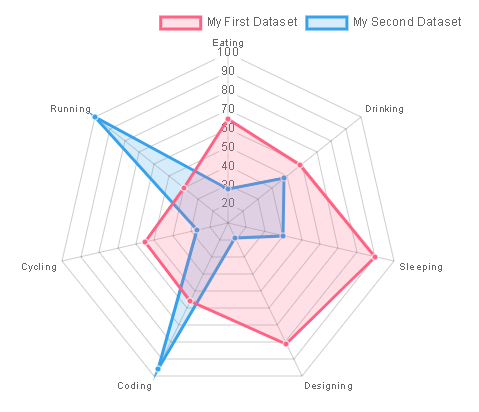
\includegraphics[scale=1]{img/radar}
			\end{center}
			\caption{Biểu đồ mạng nhện}
			\label{refhinh16}
		\end{figure}
	\end{center}
	
	\newpage
	\item Biểu đồ cột ngang (Basic bar)
	
	Biểu đồ cột ngang sẽ được áp dụng cho việc thống kê số lượng truy cập của sinh viên dựa vào những hành động mà ta muốn phân tích(VD: Số lượng sinh viên truy cập của tất cả bài kiểm tra,...).
	
	\begin{center}
		\begin{figure}[htp]
			\begin{center}
				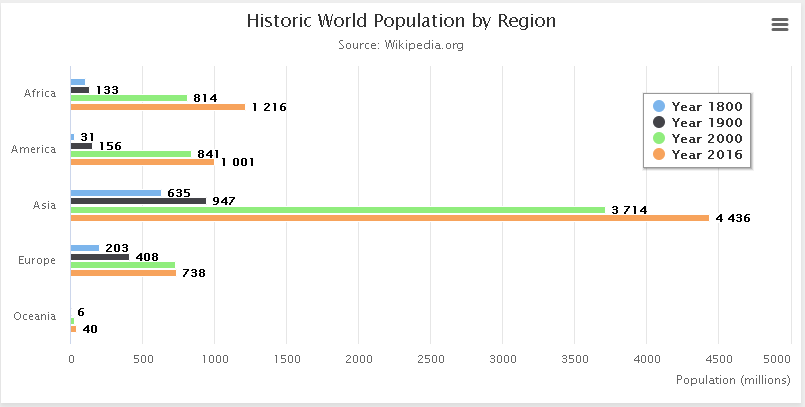
\includegraphics[scale=0.7]{img/bar}
			\end{center}
			\caption{Biểu đồ cột ngang}
			\label{refhinh17}
		\end{figure}
	\end{center}
	
	\item Biểu đồ đường (Line Chart)
	
	Biểu đồ đường được sử dụng cho việc tham khảo sự phân phối số lượt truy cập của từng sinh viên trong khóa học.
	
	\begin{center}
		\begin{figure}[htp]
			\begin{center}
				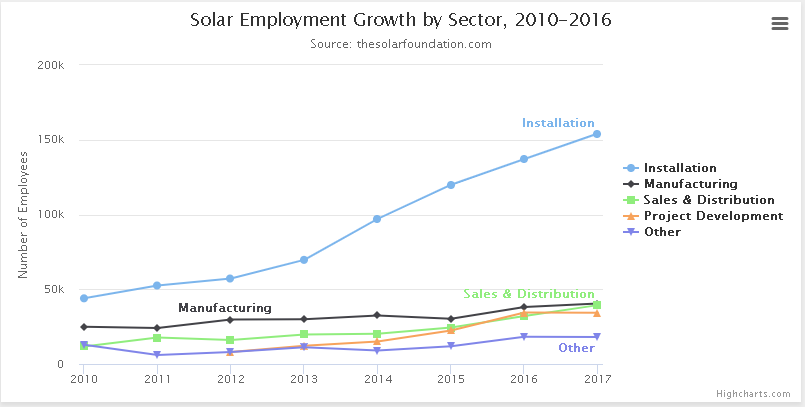
\includegraphics[scale=0.7]{img/line}
			\end{center}
			\caption{Biểu đồ đường}
			\label{refhinh18}
		\end{figure}
	\end{center}
	
\end{itemize}

	
	\newpage
	\setcounter{chapter}{3}
\chapter{Hiện thực và triển khai}

\section{Cách tạo một Khối trong Moodle \cite{createblock}}

Để tạo một Khối trong Moodle ta cần cung cấp bốn tệp PHP. Trong trường hợp này nhóm sẽ lấy khối của mình làm ví dụ minh họa cho 4 tệp này.

\subsection{Tệp block\_grades\_chart.php}

Tệp này sẽ định nghĩa lớp cho Khối và được sử dụng để quản lý Khối dưới dạng plugin và hiển thị trên màn hình.

Đầu tiên chúng ta sẽ viết hàm khởi tạo cho Khối

\begin{center}
	\begin{figure}[htp]
		\begin{center}
			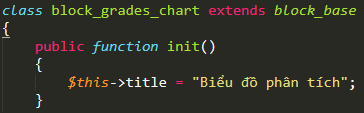
\includegraphics[scale=1]{img/initblock}
		\end{center}
		\caption{Hàm init của Khối}
		\label{refhinh22}
	\end{figure}
\end{center}

\newpage
\subsection{Tệp db/access.php}

Tiếp đến ta tạo tệp access.php nơi cung cấp các quyền truy cập của Khối

\begin{center}
	\begin{figure}[htp]
		\begin{center}
			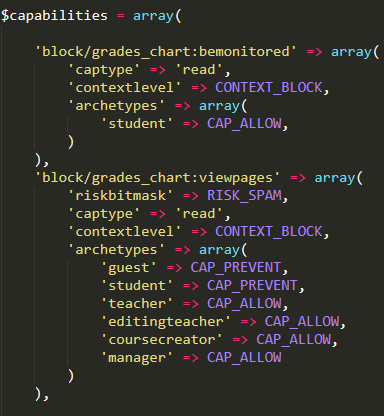
\includegraphics[scale=1]{img/capblock}
		\end{center}
		\caption{Mảng capabilities chứa những quyền truy cập vào Khối}
		\label{refhinh23}
	\end{figure}
\end{center}

\subsection{Tệp lang/en/block\_grades\_chart.php}

Tệp này sẽ chứa ngôn ngữ cho Khối của bạn. Trong phạm vi luận văn nhóm sử dụng tiếng Việt để phát triển cho Khối của mình.

\begin{center}
	\begin{figure}[htp]
		\begin{center}
			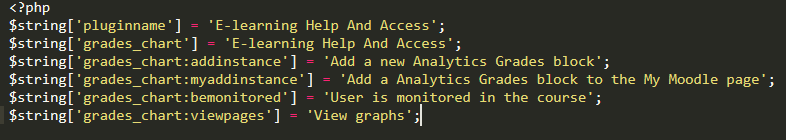
\includegraphics[scale=1]{img/langblock}
		\end{center}
		\caption{Tệp chứa ngôn ngữ cho Khối}
		\label{refhinh24}
	\end{figure}
\end{center}

\newpage
\subsection{Tệp version.php}

Tệp này chứa thông tin của Khối.

\begin{center}
	\begin{figure}[htp]
		\begin{center}
			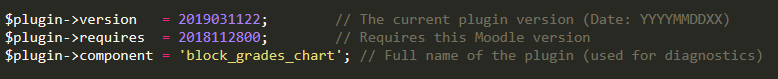
\includegraphics[scale=0.8]{img/in4block}
		\end{center}
		\caption{Thông tin của Khối}
		\label{refhinh25}
	\end{figure}
\end{center}

Trên đây là bốn tệp cơ bản để tạo ra một Khối trong Moodle. Nhưng để Khối hiển thị nội dung ra ngoài màn hình ta cần thêm một phương thức đến lớp của Khối. Code sẽ được thêm vào như sau:

\begin{center}
	\begin{figure}[htp]
		\begin{center}
			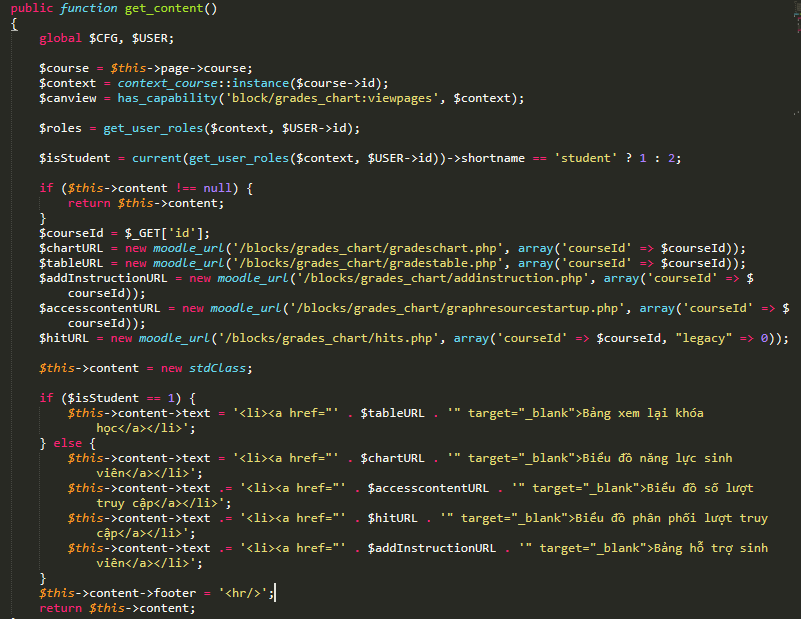
\includegraphics[scale=0.8]{img/contentblock}
		\end{center}
		\caption{Phương thức dùng để hiển thị nội dung của Khối}
		\label{refhinh26}
	\end{figure}
\end{center}

\newpage
\section{Kiến trúc của EHAT}

\begin{center}
	\begin{figure}[htp]
		\begin{center}
			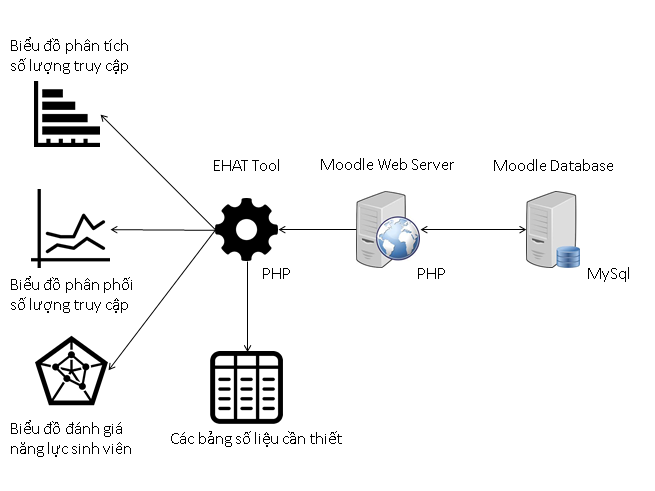
\includegraphics[scale=1]{img/kientrucehat}
		\end{center}
		\caption{Kiến trúc hệ thống EHAT}
		\label{refhinh21}
	\end{figure}
\end{center}

Trên đây là kiến trúc của EHAT trong Moodle. Tiếp đến chúng ta sẽ cùng đi tìm hiểu cách để hiện thực những chức năng của EHAT mà nhóm đã xây dựng.

\section{Hiện thực những chức năng của EHAT}

EHAT là công cụ dễ dàng để sử dụng giúp người dùng phân tích được những dữ liệu trong một khóa học trực tuyến. Bên cạnh đó EHAT còn hỗ trợ cho HV trong quá trình học tập trực tuyến.

Công cụ EHAT hiện nay sẽ hỗ trợ tổng cộng 5 chức năng chính, trong đó 4 chức năng sẽ dành cho GV còn 1 chức năng là của HS,SV. Trước tiên chúng ta sẽ cùng tìm hiểu về 4 chức năng mà EHAT cung cấp cho GV.

\subsection{Đối với GV}

EHAT sẽ cung cấp 4 chức năng chính đối với GV như hình sau:

\begin{center}
	\begin{figure}[htp]
		\begin{center}
			
\includegraphics[scale=1]{img/gvtool}
		\end{center}
		\caption{Bốn chức năng mà EHAT mang lại cho GV}
		\label{refhinh27}
	\end{figure}
\end{center}

\vskip 5cm
Trên đây là hình ảnh minh họa 4 chức năng mà EHAT mang lại cho GV, tiếp theo chúng ta sẽ cùng đi vào chi tiết từng chức năng trên xem chúng có gì hay.

Để thực hiện các chức năng này nhóm đã có tham khảo một phần source code ở \cite{code} nhằm lấy dữ liệu từ log file để vẽ biểu đồ chính xác hơn

\subsubsection{Biểu đồ đánh giá năng lực sinh viên}
\begin{itemize}
	\item Chức năng đầu tiên mà EHAT giành cho GV đó là chức năng đánh giá năng lực sinh viên. Ở chức năng này EHAT sẽ sử dụng biểu đồ mạng nhện(Spider web) để mô tả năng lực của từng cá nhân HV. Kết quả sẽ chỉ ra số điểm trung bình của các tiêu chí mà GV thiết lập để đánh giá. Bên cạnh đó còn có thêm chức năng so sánh năng lực của hai HV để thấy rõ sự khác biệt về năng lực mỗi cá nhân trong khóa học.
	
	\item Để hiện thực chức năng này nhóm đã sử dụng dữ liệu về điểm số các bài kiểm tra của sinh viên được thu thập từ bảng mdl\_quiz\_grades trong Database của Moodle đồng thời kết hợp với giá trị đầu vào như id của sinh viên, id của các bài kiểm tra,... từ đó ta tính trung bình để tìm ra được số điểm của một tiêu chí cần mô tả. Đồng thời kết hợp với biểu đồ mạng nhện được hỗ trợ bởi thư viện Highcharts để đưa giá trị ấy về dạng trực quan dễ tham khảo hơn.
\end{itemize}

\subsubsection{Biểu đồ thống kê số lượt truy cập}
\begin{itemize}
	\item Để sử dụng chức năng này đầu tiên người dùng phải chọn hạng mục mà mình muốn phân tích số liệu. Ví dụ về các hạng mục mà EHAT hỗ trợ người dùng phân tích:
	
	\begin{itemize}
		\item Bài tập lớn(Assignment)
		\item Trò chuyện(Chat)
		\item Lựa chọn(Choice)
		\item Phản hồi(Feedback)
		\item Diễn đàn(Forum)
		\item Bài giảng(Lesson)
		\item Câu hỏi(Quiz)
		\item Gói SCORM
		\item Khảo sát(Survey)
		\item Wiki
		\item Hội thảo(Workshop)
		\item Sách(Book)
		\item Tài nguyên(Resource)
		\item Tệp tin(Folder)
		\item Trang(Page)
		\item Đường dẫn(URL)
	\end{itemize}

	\item Chức năng này cho phép người dùng xem số lượt sinh viên truy cập và không truy cập của từng hạng mục cụ thể mà mình muốn phân tích. Chức năng này giúp GV thấy được mức độ hiệu quả của các tài nguyên trong khóa học để từ đó có những điều chình phù hợp cho khóa học của mình.
	
	\item Chức năng này nhóm đã đọc log file được lưu trữ trong bảng mdl\_logstore\_standard\_log của Moodle để đếm số lượng truy cập vào một mô-đun, một mô-đun được truy cập khi mô-đun đó có thể hiện hành động "viewed" hoặc "submission" được mô tả ở cột "action" và cột "instance" sẽ là cột mô tả id của mô-đun mà ta muốn tham khảo. Kèm với việc sử dụng biểu đồ cột ngang để mô tả chính xác những dữ liệu mà nhóm thu thập được.
\end{itemize}

\subsubsection{Biểu đồ phân phối lượt truy cập}
\begin{itemize}
	\item Chức năng sẽ hiển thị cho người dùng một bảng số liệu chứa những thông tin về:
	\begin{itemize}
		\item Số lần HV truy cập vào khóa học
		\item Số ngày mà HV truy cập theo tuần kèm biểu đồ mô tả
		\item Biểu đồ phần trăm lượt truy cập kèm theo đó là biểu đồ thể hiện chi tiết số lần truy cập của sinh viên
	\end{itemize}
	
	\item Bên cạnh đó bảng số liệu cũng có kèm theo dấu hiệu cho thấy HV có thường xuyên truy cập vào khóa học hay không. Để hiện thực được chức năng này ta cần lấy ra được những giá trị như sau:
	
	\begin{itemize}
		\item Số lượng ngày được truy cập trong một tuần. Dữ liệu này ta cũng sử dụng dữ liệu từ bảng mdl\_logstore\_standard\_log với điều kiện hành động của sinh viên là "viewed" và mục tiêu tác động đó là "course" và ta sẽ tính toán số tuần dựa vào ngày bắt đầu của khóa học đến thời điểm hiện tại.
		
		\item Lấy thông tin của tất cả các mô-đun được sử dụng trong khóa học thông qua bảng course\_modules của Moodle. Từ đó ta tiếp tục sử dụng bảng mdl\_logstore\_standard\_log để đếm số lần truy cập vào một mô-đun của một sinh viên đồng thời tính được số mô-đun mà sinh viên ấy truy cập và không truy cập.
	\end{itemize}
	
	Sau khi lấy được những dữ liệu như trên nhóm đã dùng bảng số liệu, biểu đồ đường, biểu đồ tròn, biểu đồ cột đứng để thể hiện các giá trị của những dữ liệu ấy.
	
\end{itemize}

\subsubsection{Bảng hỗ trợ sinh viên}
\begin{itemize}
	\item Chức năng cuối cùng mà EHAT hỗ trợ nhằm giúp cho GV thêm tài liệu tham khảo đối với mỗi câu hỏi trong mỗi bài kiểm tra. GV có thể thêm đoạn text hoặc một đường dẫn đến nơi mà mình muốn HV tham khảo. Nội dung sẽ được lưu trữ vào cơ sở dữ liệu và hiển thị cho học viên khi học viên sử dụng chức năng của EHAT.
	
	\item Chức năng này để xây dựng nhóm đã tạo thêm một bảng vào database của Moodle nhằm lưu trữ id của câu hỏi và nội dung tài liệu tham khảo. Bảng này sẽ tự động thêm vào Database khi ta thêm khối EHAT.
\end{itemize}

\subsection{Đối với HS, SV}

Hiện nay EHAT chỉ cung cấp 1 chức năng cho sinh viên:

\subsubsection{Bảng xem lại khóa học}
\begin{itemize}
	\item EHAT hiện chỉ hỗ trợ cho HS, SV chức năng xem lại toàn bộ bài các câu trả lời từ lần làm bài cuối cùng của mình. Trong đó sẽ chỉ rõ câu nào SV trả lời đúng và câu nào SV trả lời sai. Đi kèm với đó là nội dung chi tiết của từng câu hỏi và tài liệu tham khảo nhằm hỗ trợ SV học tập tốt hơn trong quá trình tự học của mình.
	
	\item Chức năng này nhóm đã lấy tất cả thông tin cần thiết của các bài kiểm tra trong lần làm bài cuối cùng của sinh viên và dữ liệu bên bảng mà nhóm đã tạo thêm để hiển thị. Tất cả thông tin ấy có trong các bảng sau:
	\begin{itemize}
		\item mdl\_quiz
		\item mdl\_question\_attempt\_steps 
		\item mdl\_question\_attempts
		\item mdl\_quiz\_grades
		\item mdl\_quiz\_slots
		\item mdl\_question
	\end{itemize}
\end{itemize}

\newpage
\section{Đặc tả yêu cầu hệ thống}

\subsection{Yêu cầu chung}

\begin{center}
	\begin{table}[!htp]
		\centering
		\begin{tabular}{|c|c|c|}
			\hline 
			STT & Nội dung & Chi tiết \\ 
			\hline 
			1 & Hệ điều hành & Ubuntu 16.04 \\ 
			\hline 
			2 & Database Server & MySQL  5.6/5.7 \\ 
			\hline 
			3 & Content Server & Apache, >= PHP 7, >= Moodle 3.6 \\ 
			\hline 
		\end{tabular} 
		\caption{Yêu cầu chung của hệ thống}
		\label{bang20}
	\end{table}
\end{center}

\subsection{EHAT đối với GV}
\subsubsection{Biểu đồ đánh giá năng lực sinh viên}
\begin{itemize}
	\item Giới thiệu: Giáo viên có thể đánh giá năng lực của từng cá nhân SV hoặc so sánh 2 SV với nhau.
	\item Inputs
	\begin{itemize}
		\item GV nhập vào số tiêu chí cần thiết lập và chọn nút "Thiết lập".
		\item GV nhập tên các tiêu chí và chọn dữ liệu cho chúng.
		\item GV chọn nút "So sánh" nếu muốn so sánh 2 SV với nhau.
		\item Chọn SV cần phân tích.
		\item Nhấn nút "Xác nhận" để xem biểu đồ.
	\end{itemize}
	\item Quy trình thực hiện
	\begin{itemize}
		\item GV nhấn chọn "Biểu đồ năng lực sinh viên" từ giao diện của Khối EHAT.
		\item GV nhập vào số tiêu chí cần thiết lập và chọn nút "Thiết lập".
		\item GV nhập tên các tiêu chí và chọn dữ liệu cho chúng.
		\item GV chọn nút "So sánh" nếu muốn so sánh 2 SV với nhau.
		\item Chọn SV cần phân tích.
		\item Nhấn nút "Xác nhận" để xem biểu đồ.
	\end{itemize}
	\item Outputs: Giao diện sẽ hiển thị biểu đồ mạng nhện thể hiện năng lực của một sinh viên hoặc so sánh 2 sinh viên mà ta đã chọn để phân tích ở trên.
	\item Xủ lí lỗi
	\begin{itemize}
		\item Nếu GV nhập số tiêu chí ít hơn 3 thì sẽ hiển thị thông báo lỗi và yêu cầu GV nhập lại.
		\item Nếu tên các tiêu chí hoặc dữ liệu của chúng chưa được thêm thì sẽ hiển thị thông báo yêu cầu GV nhập.
		\item Nếu 2 SV so sánh là như nhau thì sẽ hiển thị thông báo lỗi.
	\end{itemize}
\end{itemize}

\subsubsection{Biểu đồ thống kê số lượt truy cập}
\begin{itemize}
	\item Giới thiệu: Giáo viên sử dụng biểu đồ để quan sát số lượng SV tương tác với một hạng mục trong khóa học.
	\item Inputs
	\begin{itemize}
		\item Chọn hạng mục cần tham khảo(Có thể nhấn nút chọn tất cả để xem hết tất cả các hạng mục).
		\item Thiết lập thời gian bắt đầu.
		\item Nhấn nút "Xem biểu đồ" để hiển thị kết quả.
	\end{itemize}
	\item Quy trình thực hiện
	\begin{itemize}
		\item GV nhấn chọn "Biểu đồ thống kê số lượt truy cập" từ giao diện của Khối EHAT
		\item GV sẽ chọn hạng mục cần tham khảo(Có thể nhấn nút chọn tất cả để xem hết tất cả các hạng mục).
		\item GV thiết lập thời gian bắt đầu.(Thời gian mặc định là ngày khóa học bắt đầu).
		\item Nhấn nút "Xem biểu đồ" để hiển thị kết quả.
	\end{itemize}
	\item Outputs: Giao diện sẽ hiển thị biểu đồ cột ngang thể hiện tất cả số lượt truy cập và không truy cập của SV đối với từng hạng mục mà ta đã chọn. Đồng thời hiển thị thêm chi tiết SV nào truy cập hay không truy cập trong hạng mục đó.
	\item Xủ lí lỗi
	\begin{itemize}
		\item Nếu GV không chọn hạng mục thì sẽ hiển thị thông báo lỗi.
	\end{itemize}
\end{itemize}
\subsubsection{Biểu đồ phân phối lượt truy cập}
\begin{itemize}
	\item Giới thiệu: GV dùng để xem xét chi tiết mức độ tương tác của từng cá nhân HS, SV đối với các tài nguyên trong quá trình học.
	\item Inputs: 
	\begin{itemize}
		\item Chọn mục "Biểu đồ phân phối lượt truy cập" từ giao diện của Khối EHAT
		\item Di chuyển chuột vào các điểm trên biểu đồ đường để xem số ngày truy cập trong tuần của sinh viên.
		\item Nhấp vào tên của sinh viên để hiển thị giao diện biểu đồ chi tiết của sinh viên ấy.
		\item Ở giao diện biểu đồ chi tiết của sinh viên chọn mục "Chi tiết lượt truy cập" để xem mức độ tương tác tài nguyên trong khóa học của sinh viên.
		\item Nhấp chọn vùng "Truy cập" để hiển thị biểu đồ chi tiết số lần truy cập của sinh viên đối với các tài nguyên tương ứng
	\end{itemize}
	\item Quy trình thực hiện: Chọn mục "Biểu đồ phân phối lượt truy cập" từ giao diện của Khối EHAT
	\item Outputs: Kết quả sẽ hiển thị bảng số liệu và các biểu đồ tương ứng chứa tất cả thông tin hoạt động của từng cá nhân HS, SV trong khóa học.
	\item Xủ lí lỗi: N/A
\end{itemize}
\subsubsection{Bảng hỗ trợ sinh viên}
\begin{itemize}
	\item Giới thiệu: Giúp GV thêm nguồn tài liệu tham khảo cho HS, SV.
	\item Inputs
	\begin{itemize}
		\item GV chọn nút "Thêm hướng dẫn".
		\item GV chọn câu hỏi cần thêm tham khảo và nhập nội dung tham khảo vào câu hỏi đó.
		\item Nhấn nút "Xác nhận" để thêm tài liệu tham khảo.
	\end{itemize}
	\item Quy trình thực hiện
	\begin{itemize}
		\item GV nhấn chọn "Bảng hỗ trợ sinh viên" từ giao diện của Khối EHAT
		\item GV chọn nút "Thêm hướng dẫn".
		\item GV chọn câu hỏi cần thêm tham khảo và nhập nội dung tham khảo vào câu hỏi đó.
		\item Nhấn nút "Xác nhận" để thêm tài liệu tham khảo.
	\end{itemize}
	\item Outputs: Nội dung tham khảo sẽ được thêm vào database để hỗ trợ SV.
	\item Xủ lí lỗi: N/A
\end{itemize}

\subsection{EHAT đối với HS, SV}
\subsubsection{Bảng xem lại khóa học}
\begin{itemize}
	\item Giới thiệu: Giúp SV xem lại kết quả của các bài kiểm tra của mình trong khóa học.
	\item Inputs: SV nhấn chọn "Bảng xem lại khóa học" từ giao diện của Khối EHAT
	\item Quy trình thực hiện: SV nhấn chọn "Bảng xem lại khóa học" từ giao diện của Khối EHAT
	\item Outputs: Công cụ sẽ hiển thị ra bảng kết quả chứa tất cả thông tin về câu trả lời của SV trong quá trình kiểm tra.
	\item Xủ lí lỗi: N/A
\end{itemize}
	
	\newpage
	\setcounter{chapter}{4}
\chapter{Kết quả}
	
	\newpage
	\setcounter{chapter}{5}
\chapter{Kết luận và hướng phát triển}

\section{Kết luận}
Trải qua khoảng thời gian đề cương luận văn và cả luận văn tốt nghiệp, chúng em đã tiếp thu cũng như học hỏi được thêm nhiều kiến thức về việc phân tích, xây dựng nên một công cụ kèm theo đó là tăng khả năng lập trình. Những kỹ năng này thật sự rất bổ ích, cần thiết cho nhóm chúng em để làm kiến thức chuẩn bị cho công việc sau này.

Về chuyên môn, nhóm chúng em đã phần nào xây dựng được công cụ nhằm giải quyết được yêu cầu đặt ra ban đầu. Sau đây là đánh giá cho từng phần trong luận văn mà nhóm đã làm được một cách cụ thể:

\begin{itemize}
	\item Phần 1: Công cụ EHAT đối với GV.
	Phần này được chia làm 4 chức năng chính, trong những chức năng đó vẫn còn có những hạn chế mà nhóm chưa cải thiện được trong quá trình luận văn này
	\begin{itemize}
		\item Chức năng đầu tiên mà nhóm kể đến đó là EHAT có thể được sử dụng để đánh giá chi tiết và so sánh năng lực của sinh viên thông qua biểu đồ mạng nhện. 
		
		Tuy vậy chức năng này vẫn còn mặt hạn chế đó là việc tính toán số điểm của từng tiêu chí mỗi sinh viên chưa thật sự đa dạng chỉ dựa vào điểm trung bình các tiêu chí mà GV chọn lựa.
		
		\item Chức năng thứ hai mà nhóm làm được là biểu đồ cột ngang nhằm thống kê số lượt truy cập của sinh viên vào một hạng mục cụ thể. 
		
		Hiện ở chức năng này nhóm vẫn chưa cải thiện được giao diện cũng như dữ liệu hiện ra vẫn còn chưa tối giản.
		
		\item Biểu đồ phân phối lượt truy cập của từng cá nhân HS, SV là chức năng thứ ba mà nhóm muốn nói. Dựa vào biểu đồ này GV có thể thấy được thái độ học tập của mỗi HV trong khóa học. 
		
		Mặt hạn chế của chức năng này đó là nhóm vẫn chưa hiển thị được thời gian mà HV truy cập vào tài nguyên.
		
		\item Chức năng cuối cùng đó là bảng hỗ trợ cho GV thêm tài liệu tham khảo của mình để HV có thể thấy và tham khảo. 
		
		Tuy vậy chức năng này còn đang hoạt động một cách thủ công chưa được tự động.
	\end{itemize}
	\item Phần 2: Công cụ EHAT đối với HS, SV
	
	Đối với HS, SV bởi nhóm chưa nghĩ ra được thêm chức năng nào khác dành cho HS, SV nên hiện tại nhóm chỉ làm được một chức năng đó là bảng số liệu nhằm giúp HV tham khảo lại chi tiết bài kiểm tra cuối cùng của mình, bên cạnh đó có hiển thị thông tin nội dung tham khảo mà GV đã thêm vào.
	
	Hạn chế của chức năng này hiện vẫn còn hạn chế đó là HS chỉ được tham khảo lại chi tiết bài kiểm tra cuối cùng mà không xem được các bài kiểm tra của những lần khác, giao diện vẫn còn đơn giản chưa thật sự bắt mắt.
\end{itemize}

\section{Hướng phát triển}

Để sản phẩm được hoàn thiện hơn thì nhóm sẽ cải thiện về những mặt sau đây:

\begin{itemize}
	\item Ngoài việc tính điểm dựa trên việc lấy trung bình nhóm sẽ nghiên cứu và thêm nhiều thuật toán hơn để tính điểm của từng tiêu chí để đánh giá một cách chính xác hơn từng cá nhân sinh viên.
	
	\item Cải thiện về mặt giao diện với từng chức năng mà nhóm đã hiện thực.
	
	\item Ở phần hiển thị chi tiết số lần truy cập của sinh viên đối với một tài nguyên cụ thể nhóm sẽ tiếp tục xây dựng để hiển thị thêm khoảng thời gian mà sinh viên ấy tương tác với tài nguyên là lúc nào để GV đánh giá thói quen học tập của SV chính xác hơn.
	
	\item Cải thiện chức năng cuối cùng mà EHAT dành cho GV để việc thêm tài liệu sẽ hoạt động một cách tự động nhằm tiết kiệm thời gian cho GV.
	
	\item Nghiên cứu và xây dựng thêm những chức năng để hỗ trợ cho SV.
	
	\item Phát triển thêm để công cụ có thể tự xây dựng khóa học phù hợp dành riêng cho từng cá nhân sinh viên.
\end{itemize}

\section{Lời kết}

Trải qua khoảng thời gian hai học kỳ của đề cương và làm luận văn nhóm chúng em thật sự rất cảm kích, biết ơn đến tất cả các thầy cô đã dạy dỗ, truyền đạt những kiến thức cần thiết để chúng em có thể thực hiện tốt đề tài của thầy Thoại Nam. Bên cạnh đó luận văn cũng đã giúp chúng em có cái nhìn rộng hơn về việc phân tích, xây dựng một công cụ, một ứng dụng phục vụ cho một nhu cầu nào đó. 

Một lần nữa, chúng em xin cảm ơn thầy Thoại Nam dù biết thầy rất bận rộn với công việc của mình nhưng thầy vẫn luôn gắn bó với tụi em trong suốt giai đoạn từ đề cương cho đến luận văn. Cám ơn thầy đã cho chúng em thử thách cuối cùng thật ý nghĩa này trước khi chúng em bước ra trải nghiệm môi trường thực tế đầy những khó khăn phải đối mặt. 

Cảm ơn Bách Khoa nơi đã mang đến cho chúng em một môi trường gian khổ nhưng vui vẻ, hạnh phúc.
	
	\clearpage
	\phantomsection
	\addcontentsline{toc}{chapter}{Tài liệu tham khảo}
	\printbibliography
	
	\clearpage
	\phantomsection
	\addcontentsline{toc}{chapter}{Phụ lục}
	\section{Hướng dẫn sử dụng công cụ EHAT}

Trước khi đi vào tìm hiểu giao diện của công cụ EHAT chúng ta cần điểm sơ qua các bước để cài đặt Moodle và cách để cài đặt một Khối trong Moodle.

\subsection{Các bước cài đặt nền tảng Moodle}

\subsubsection{Tải về gói cài đặt Moodle}

\begin{center}
	\begin{figure}[htp]
		\begin{center}
			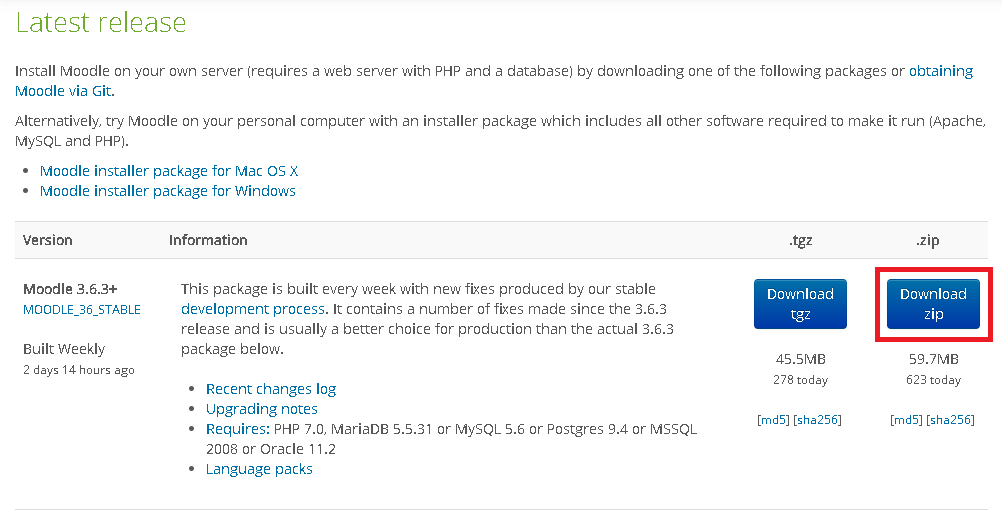
\includegraphics[width=0.8\linewidth]{img/packagemoodle}
		\end{center}
		\caption{Gói cài đặt Moodle 3.6.3+}
		\label{refhinh28}
	\end{figure}
\end{center}

\subsubsection{Tạo một cơ sở dữ liệu có tên moodle trên phpMyAdmin}

\begin{center}
	\begin{figure}[htp]
		\begin{center}
			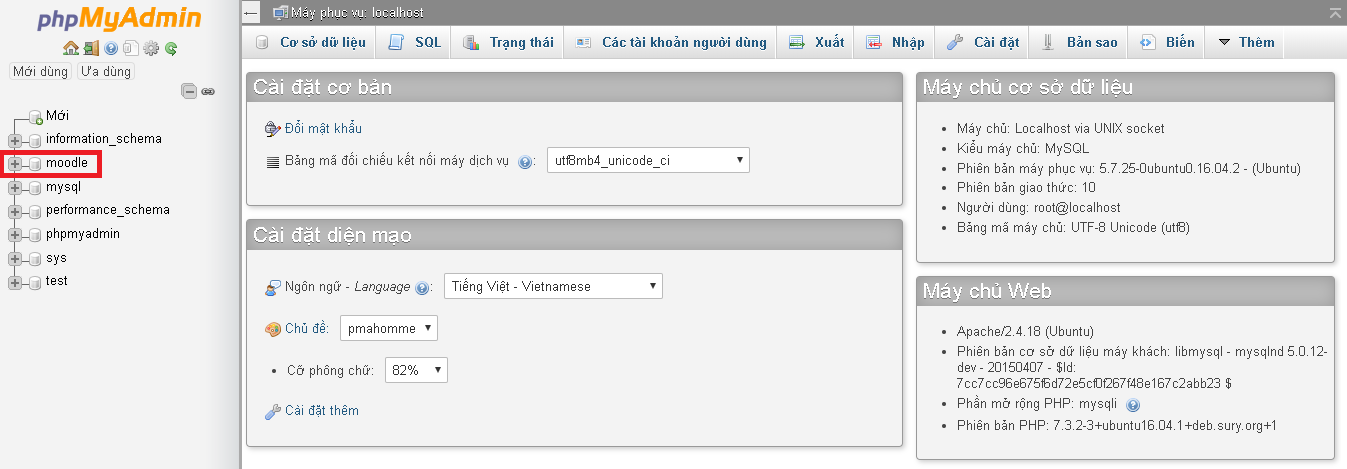
\includegraphics[width=1.3\linewidth]{img/dbmoodle}
		\end{center}
		\caption{Cơ sở dữ liệu moodle}
		\label{refhinh29}
	\end{figure}
\end{center}

\newpage
\subsubsection{Quá trình cài đặt Moodle}

\begin{center}
	\begin{figure}[htp]
		\begin{center}
			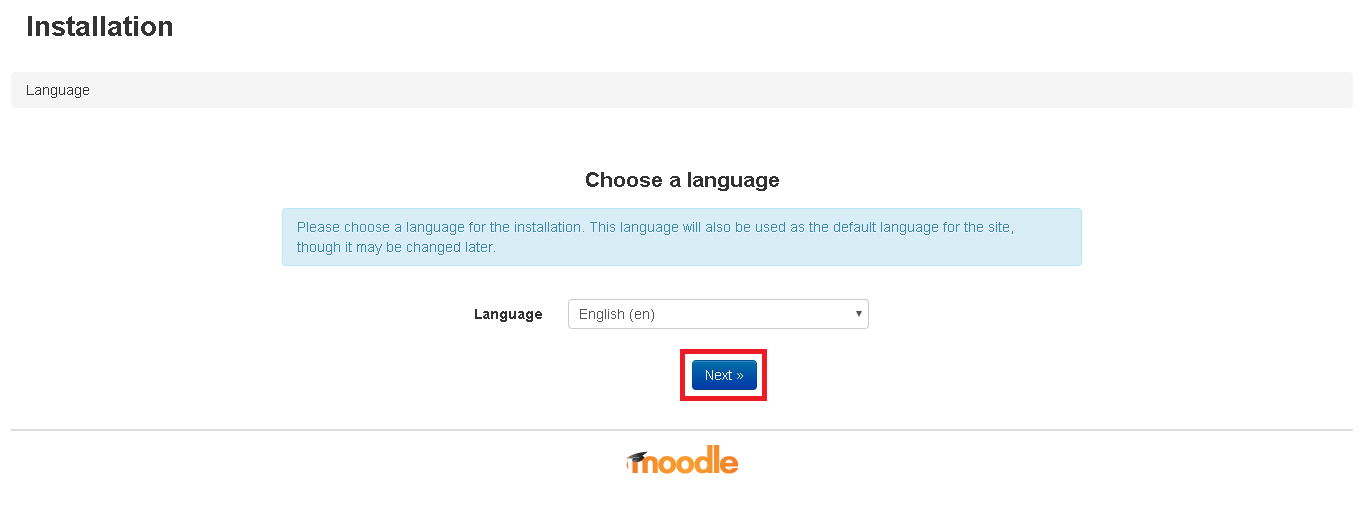
\includegraphics[width=1\linewidth]{img/choosenn}
		\end{center}
		\caption{Chọn ngôn ngữ cho Moodle}
		\label{refhinh30}
	\end{figure}
\end{center}

\begin{center}
	\begin{figure}[htp]
		\begin{center}
			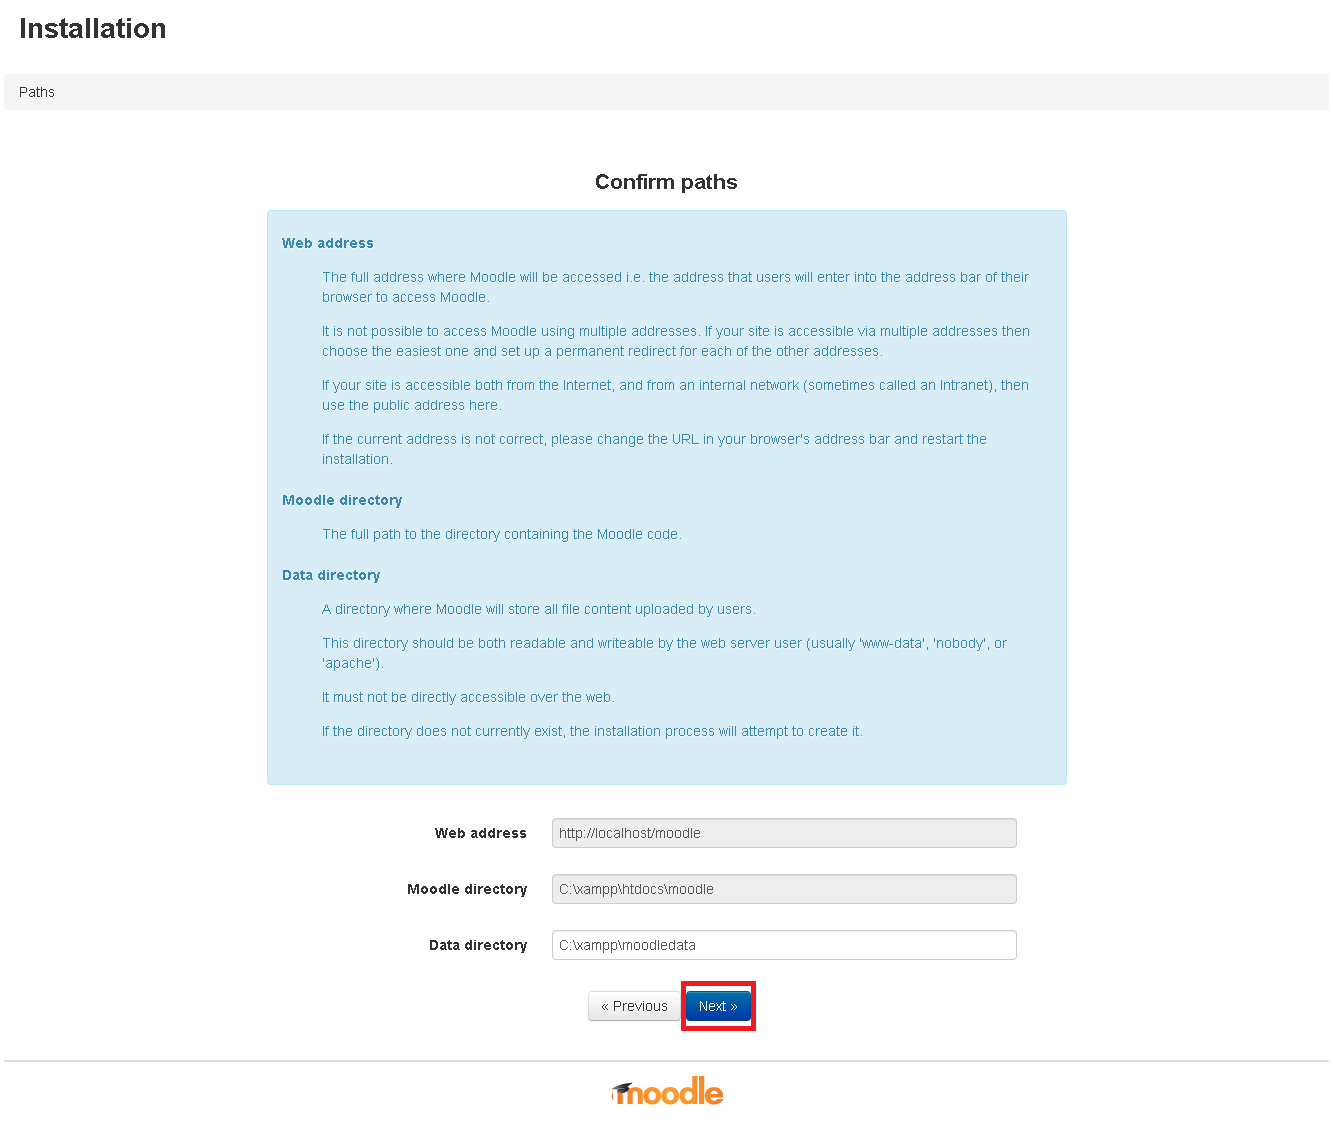
\includegraphics[width=0.8\linewidth]{img/direct}
		\end{center}
		\caption{Xác định lại các địa chỉ}
		\label{refhinh31}
	\end{figure}
\end{center}

\begin{center}
	\begin{figure}[htp]
		\begin{center}
			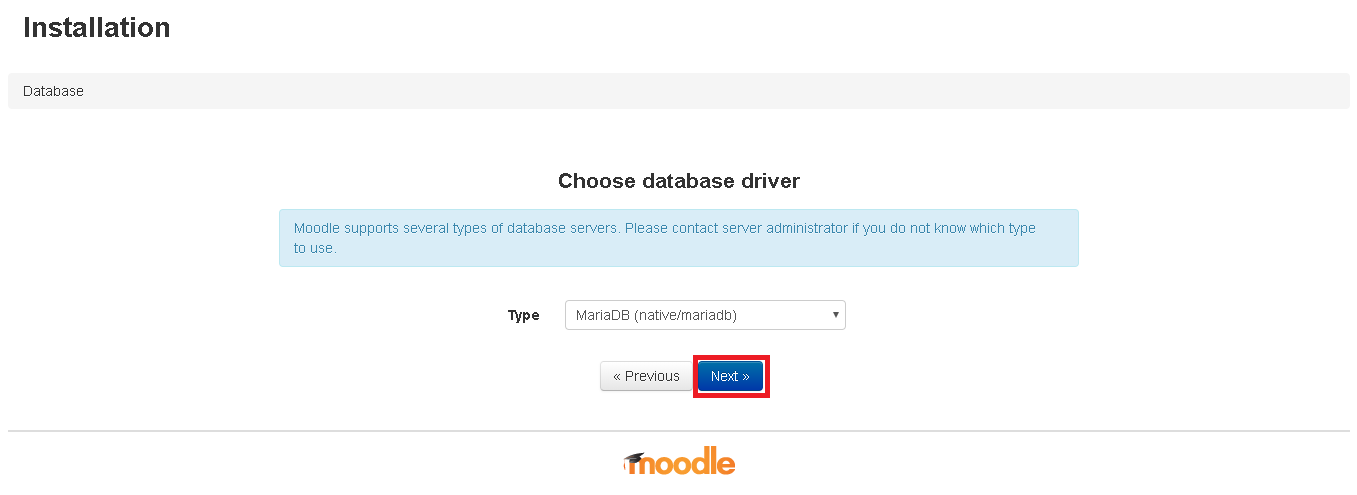
\includegraphics[width=1\linewidth]{img/2}
		\end{center}
		\caption{Chọn loại cơ sở dữ liệu}
		\label{refhinh32}
	\end{figure}
\end{center}

\begin{center}
	\begin{figure}[htp]
		\begin{center}
			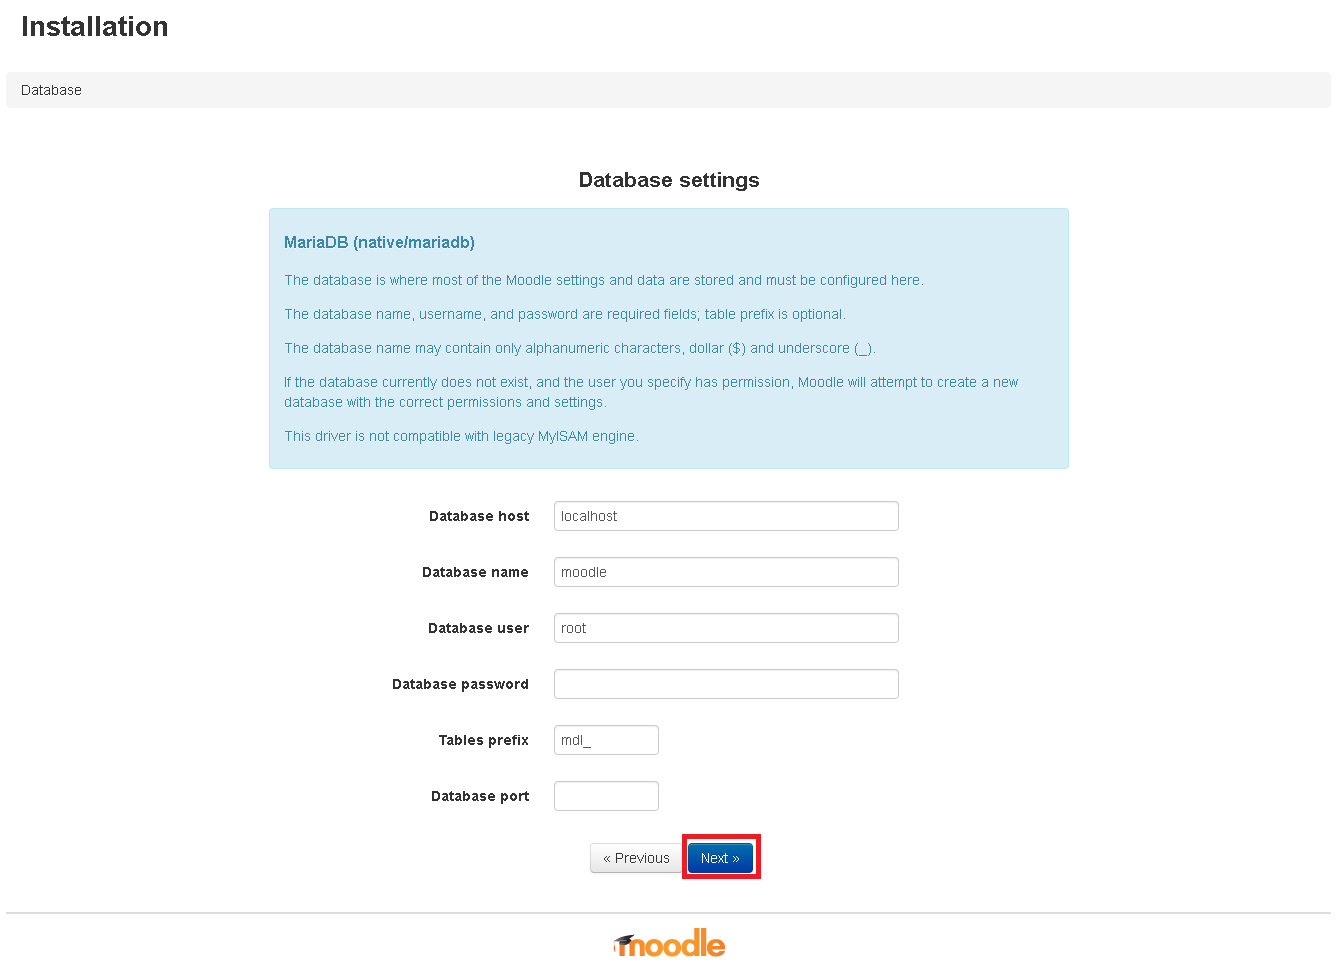
\includegraphics[width=1\linewidth]{img/3}
		\end{center}
		\caption{Cấu hình cơ sở dữ liệu}
		\label{refhinh33}
	\end{figure}
\end{center}

\begin{center}
	\begin{figure}[htp]
		\begin{center}
			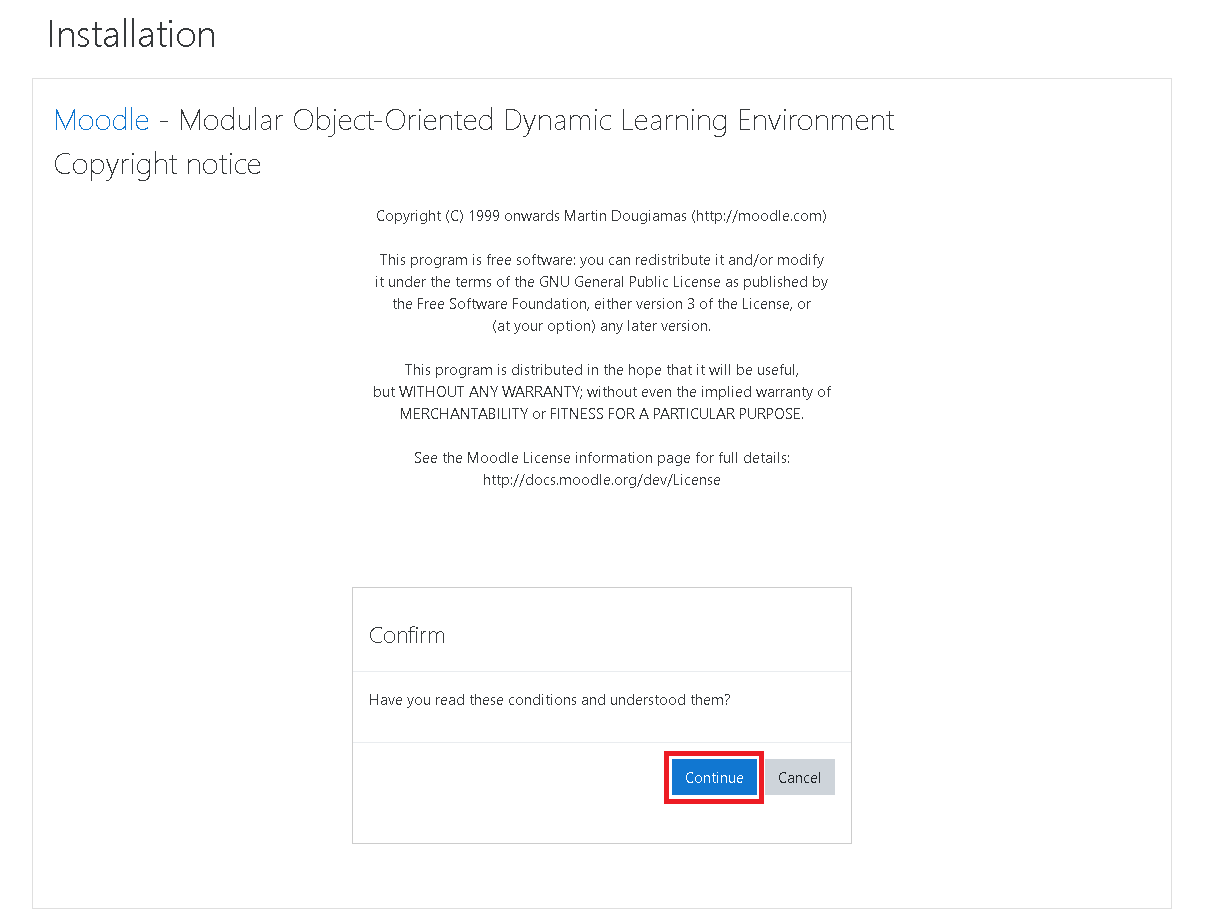
\includegraphics[width=0.8\linewidth]{img/4}
		\end{center}
		\caption{Điều kiện của Moodle}
		\label{refhinh34}
	\end{figure}
\end{center}

\begin{center}
	\begin{figure}[htp]
		\begin{center}
			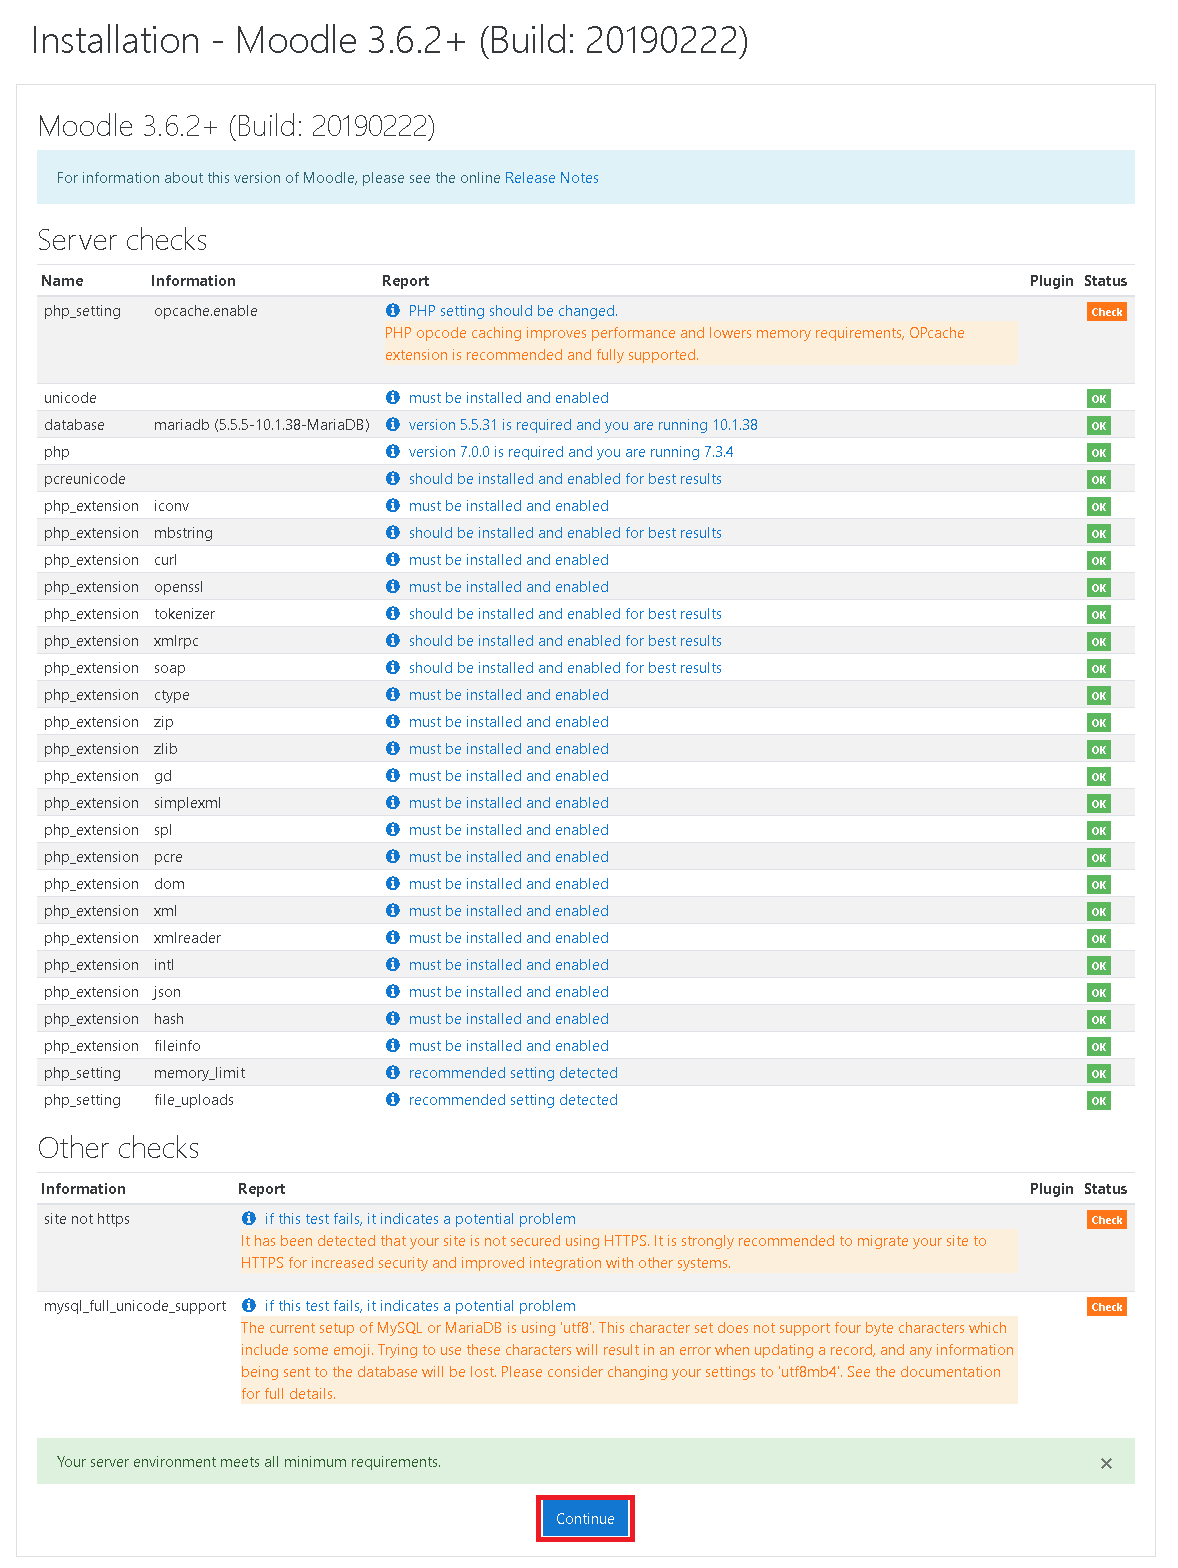
\includegraphics[width=0.65\linewidth]{img/5}
		\end{center}
		\caption{Kiểm tra server}
		\label{refhinh35}
	\end{figure}
\end{center}

\vskip 9cm
Chờ trong giây lát quá trình cài đặt Moodle sẽ hoàn thành.

\subsection{Cài đặt Khối EHAT}
Tiếp theo nhóm sẽ giới thiệu quá trình cài đặt công cụ EHAT. Hãy kiểm tra lại lần nữa là Moodle của bạn đã được cài đặt và hoạt động bình thường nếu vẫn chưa cài Moodle thì hãy xem lại mục 4.3.1. Quá trình cài đặt sẽ được mô tả theo các bước sau:

\begin{itemize}
	\item Tại giao diện chính của trang chủ chọn mục Quản trị hệ thống(Đăng nhập Moodle với quyền Admin).
	
	\begin{center}
		\begin{figure}[htp]
			\begin{center}
				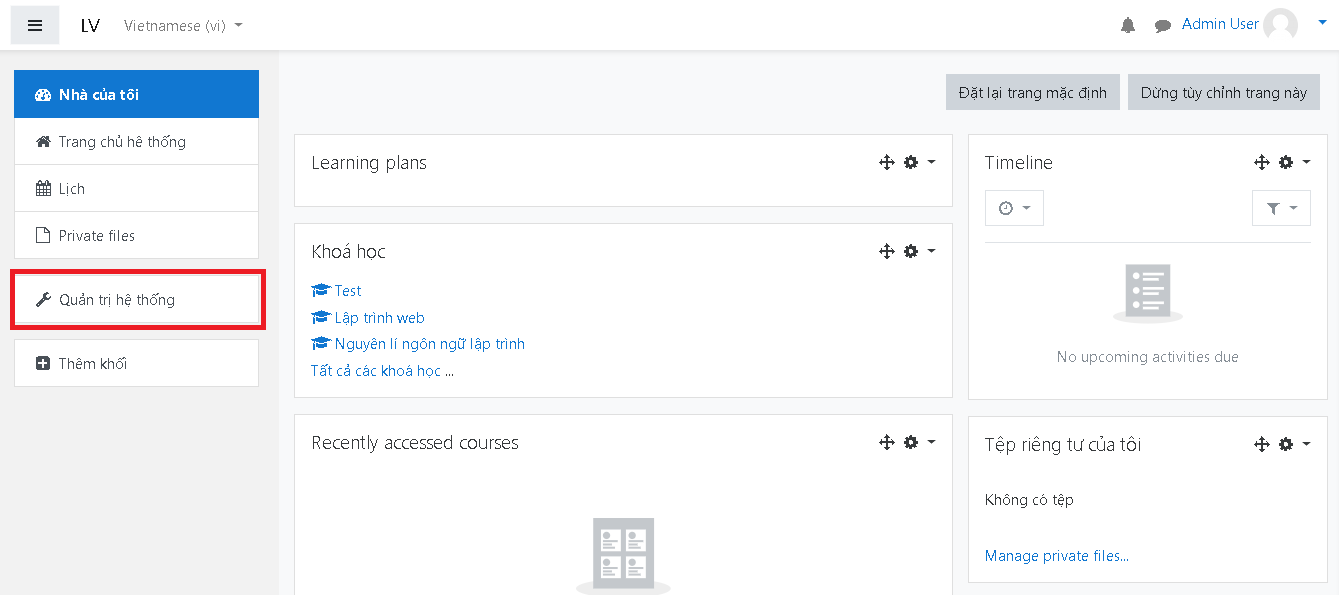
\includegraphics[width=1\linewidth]{img/6}
			\end{center}
			\caption{Chọn chức năng quản trị hệ thống}
			\label{refhinh36}
		\end{figure}
	\end{center}
	
	\item Tại trang Quản trị hệ thống người dùng chọn mục Module và chọn Install plugins
	
	\begin{center}
		\begin{figure}[htp]
			\begin{center}
				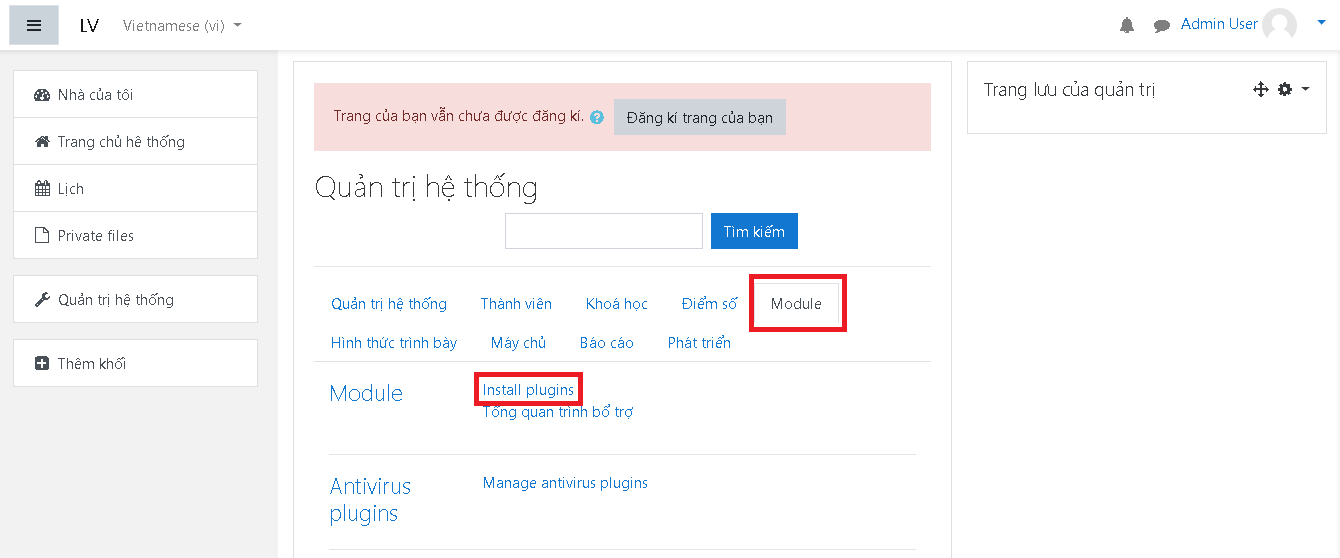
\includegraphics[width=1\linewidth]{img/7}
			\end{center}
			\caption{Chọn install plugins}
			\label{refhinh37}
		\end{figure}
	\end{center}
	
	\newpage
	\item Kéo thả tệp tin chứa công cụ EHAT(Định dạng file .zip).
	
	\begin{center}
		\begin{figure}[htp]
			\begin{center}
				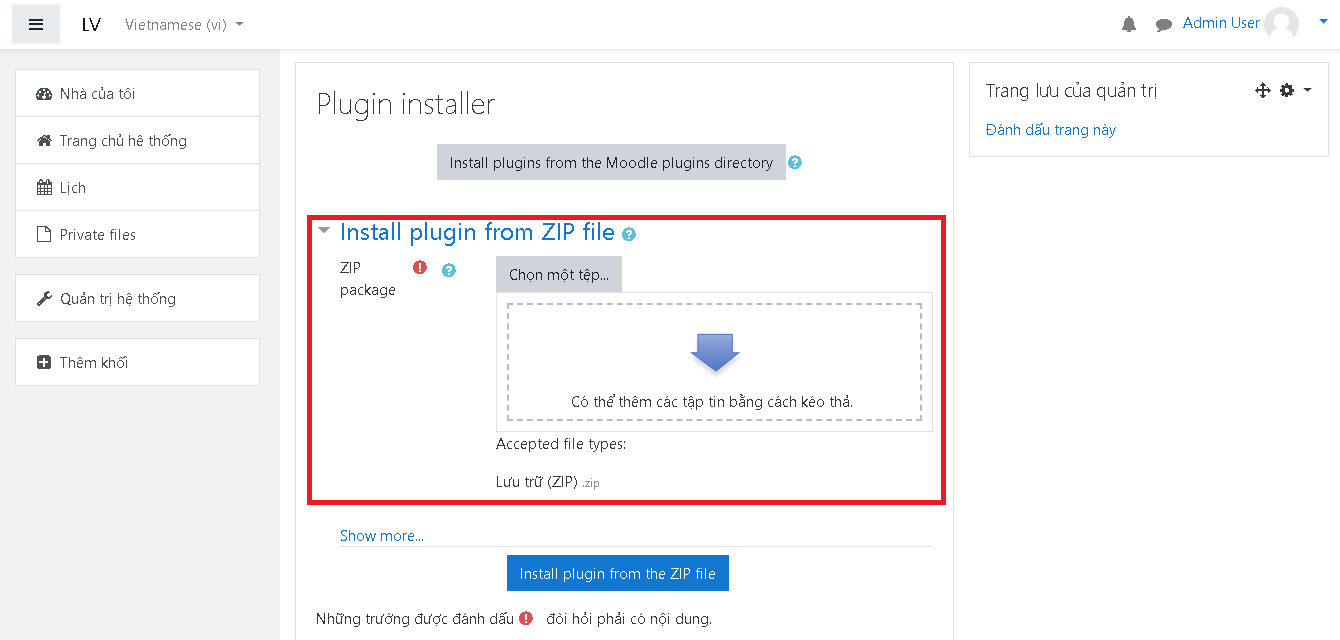
\includegraphics[width=1\linewidth]{img/8}
			\end{center}
			\caption{Chọn tệp tin chứa công cụ EHAT}
			\label{refhinh38}
		\end{figure}
	\end{center}
	
	\item Chọn Install plugin để tiếp tục.
	
	\begin{center}
		\begin{figure}[htp]
			\begin{center}
				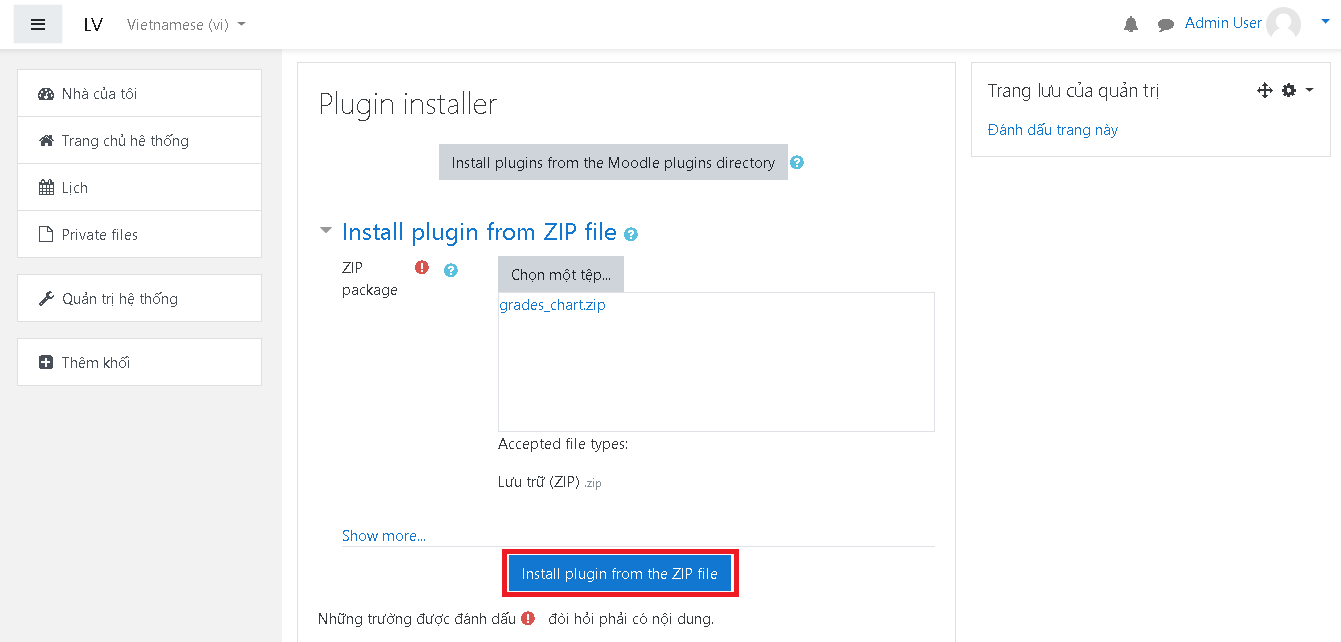
\includegraphics[width=1\linewidth]{img/9}
			\end{center}
			\caption{Chọn Install plugin để tiếp tục}
			\label{refhinh39}
		\end{figure}
	\end{center}
	
	\newpage
	\item Tiếp tục để cài đặt công cụ.
	
	\begin{center}
		\begin{figure}[htp]
			\begin{center}
				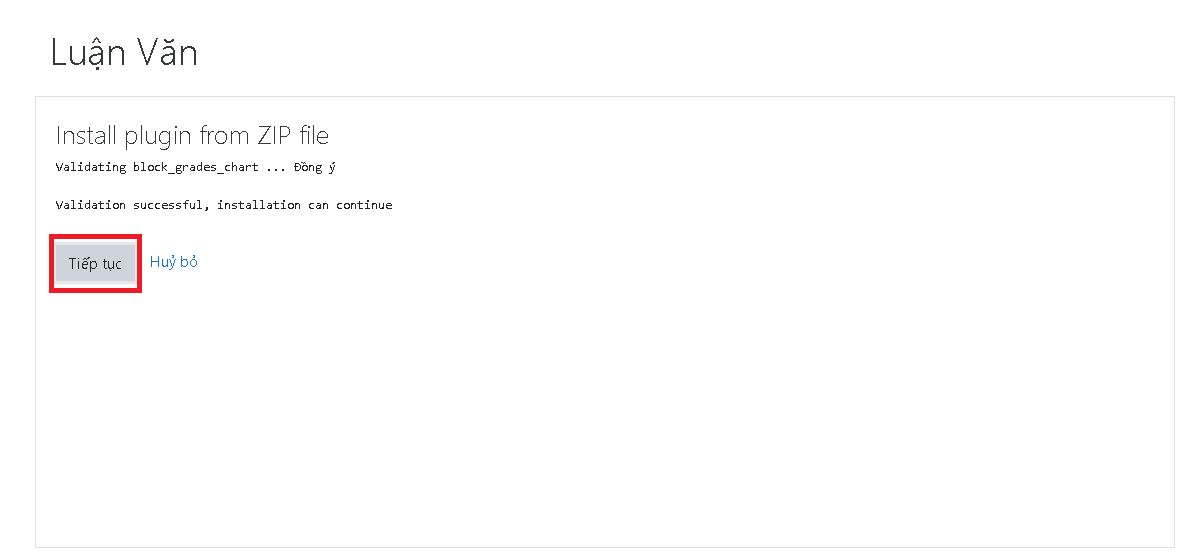
\includegraphics[width=1\linewidth]{img/10}
			\end{center}
			\caption{Chọn tiếp tục}
			\label{refhinh40}
		\end{figure}
	\end{center}
	
	\item Nâng cấp cơ sở dữ liệu Moodle để hoàn tất quá trình cài đặt
	
	\begin{center}
		\begin{figure}[htp]
			\begin{center}
				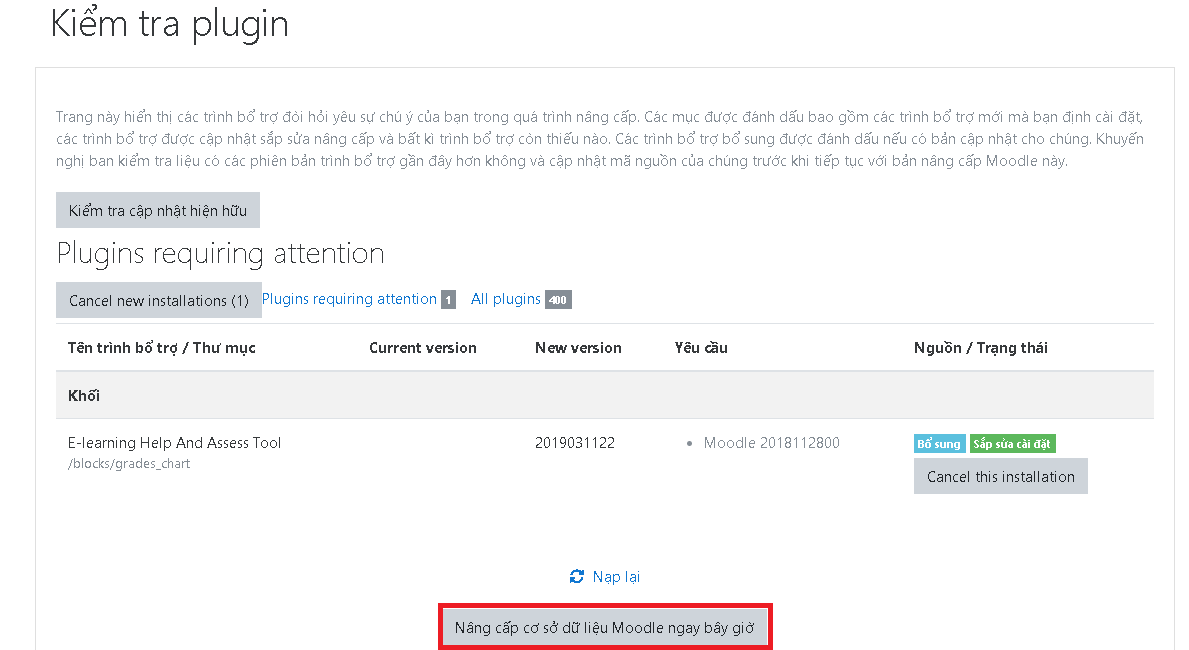
\includegraphics[width=1\linewidth]{img/11}
			\end{center}
			\caption{Giao diện nâng cấp cơ sở dữ liệu}
			\label{refhinh41}
		\end{figure}
	\end{center}
	
	\vskip 5cm
	\item Hoàn tất quá trình cài đặt EHAT
	
	\begin{center}
		\begin{figure}[htp]
			\begin{center}
				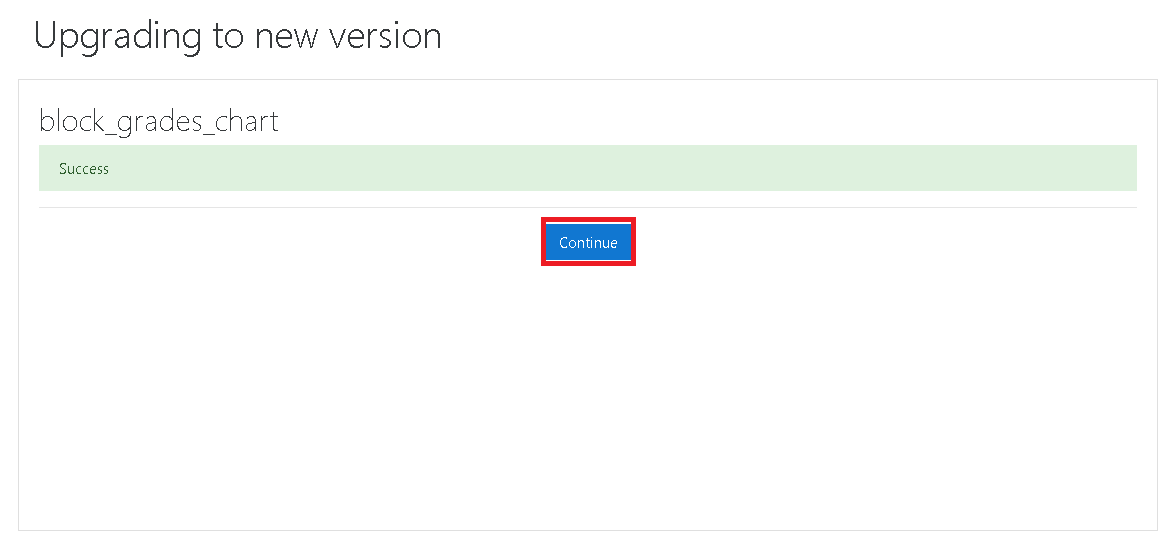
\includegraphics[width=1\linewidth]{img/12}
			\end{center}
			\caption{Quá trình cài đặt hoàn thành}
			\label{refhinh42}
		\end{figure}
	\end{center}
	
\end{itemize}


\subsection{Các chức năng của EHAT đối với GV}

Đầu tiên để thấy được các chức năng của EHAT chúng ta cần thêm công cụ EHAT vào một khóa học mà ta muốn phân tích.

Ở giao diện trang chủ của Moodle ta chọn khóa học mà mình muốn thêm công cụ EHAT.

\begin{center}
	\begin{figure}[htp]
		\begin{center}
			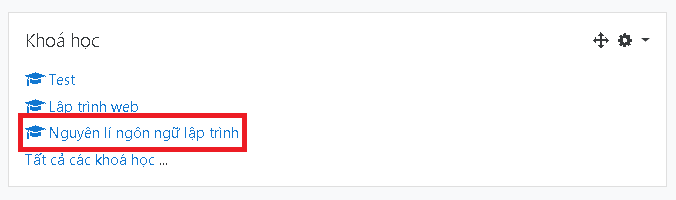
\includegraphics[width=1\linewidth]{img/35}
		\end{center}
		\caption{Chọn khóa học muốn phân tích}
		\label{refhinh43}
	\end{figure}
\end{center}

\newpage
Bật chế độ chỉnh sửa trong khóa học và chọn mục Thêm khối.

\begin{center}
	\begin{figure}[htp]
		\begin{center}
			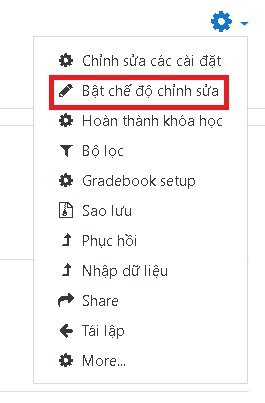
\includegraphics[width=0.4\linewidth]{img/36}
		\end{center}
		\caption{Bật chế độ chỉnh sửa}
		\label{refhinh44}
	\end{figure}
\end{center}

\begin{center}
	\begin{figure}[htp]
		\begin{center}
			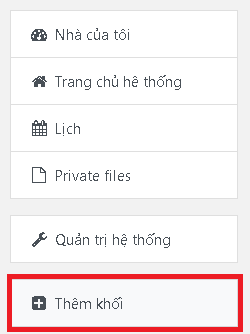
\includegraphics[width=0.35\linewidth]{img/38}
		\end{center}
		\caption{Chọn Thêm khối}
		\label{refhinh46}
	\end{figure}
\end{center}

\newpage
Chọn khối E-learning Help And Assess Tool

\begin{center}
	\begin{figure}[htp]
		\begin{center}
			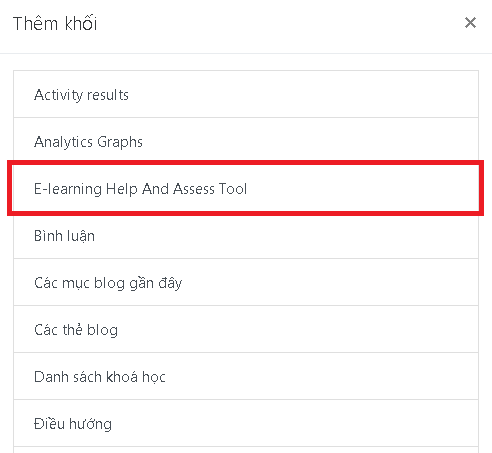
\includegraphics[width=0.6\linewidth]{img/37}
		\end{center}
		\caption{Chọn khối EHAT}
		\label{refhinh45}
	\end{figure}
\end{center}

Như vậy ta đã thêm công cụ EHAT vào khóa học.

\begin{center}
	\begin{figure}[htp]
		\begin{center}
			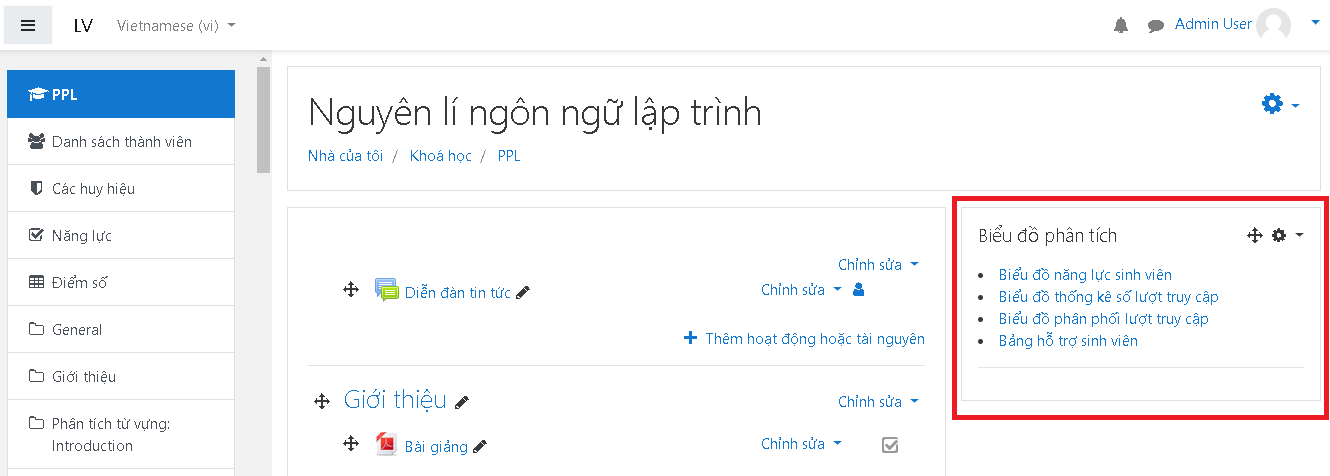
\includegraphics[width=1\linewidth]{img/39}
		\end{center}
		\caption{Thêm EHAT thành công}
		\label{refhinh47}
	\end{figure}
\end{center}

\newpage
\subsubsection{Chức năng đánh giá năng lực SV}

Chúng ta cùng tìm hiểu giao diện của chức năng đầu tiên mà EHAT cung cấp cho GV.

\begin{center}
	\begin{figure}[htp]
		\begin{center}
			
\includegraphics[width=1\linewidth]{img/16}
		\end{center}
		\caption{Màn hình chính của chức năng thứ nhất}
		\label{refhinh48}
	\end{figure}
\end{center}

Nếu nhập số tiêu chí ít hơn 3 sẽ hiện thông báo lỗi.

\begin{center}
	\begin{figure}[htp]
		\begin{center}
			
\includegraphics[width=1\linewidth]{img/17}
		\end{center}
		\caption{Thông báo lỗi 1}
		\label{refhinh49}
	\end{figure}
\end{center}

\newpage
Nếu ta nhập đúng số tiêu chí thì giao diện sẽ chuyển sang màn hình mới.

\begin{center}
	\begin{figure}[htp]
		\begin{center}
			\includegraphics[width=0.6\linewidth]{img/18}
		\end{center}
		\caption{Màn hình thiết lập biểu đồ}
		\label{refhinh50}
	\end{figure}
\end{center}

Nếu ta không nhập tên tiêu chí hoặc thêm dữ liệu cho tiêu chí thì EHAT cũng sẽ báo lỗi.
\begin{center}
	\begin{figure}[htp]
		\begin{center}
			\includegraphics[width=0.6\linewidth]{img/19}
		\end{center}
		\caption{Thông báo lỗi 2}
		\label{refhinh51}
	\end{figure}
\end{center}

\begin{center}
	\begin{figure}[htp]
		\begin{center}
			\includegraphics[width=0.6\linewidth]{img/20}
		\end{center}
		\caption{Thông báo lỗi 3}
		\label{refhinh52}
	\end{figure}
\end{center}

\vskip 5cm
Màn hình chọn dữ liệu cho tiêu chí.

\begin{center}
	\begin{figure}[htp]
		\begin{center}
			\includegraphics[width=0.5\linewidth]{img/21}
		\end{center}
		\caption{Giao diện chọn dữ liệu}
		\label{refhinh53}
	\end{figure}
\end{center}

\newpage
Sau khi đã hoàn tất mọi yêu cầu, chọn sinh viên cần tham khảo và nhấn nút xác nhận để xem biểu đồ năng lực của sinh viên đó.

\begin{center}
	\begin{figure}[htp]
		\begin{center}
			\includegraphics[width=1\linewidth]{img/22}
		\end{center}
		\caption{Biểu đồ năng lực sinh viên Nguyễn Anh Tuấn}
		\label{refhinh54}
	\end{figure}
\end{center}

\subsubsection{Chức năng so sánh năng lực 2 SV}

Chọn nút So sánh nếu muốn so sánh 2 SV với nhau.

\begin{center}
	\begin{figure}[htp]
		\begin{center}
			\includegraphics[width=0.4\linewidth]{img/23}
		\end{center}
		\caption{So sánh 2 SV}
		\label{refhinh55}
	\end{figure}
\end{center}
\vskip 3cm

Thông báo lỗi sẽ hiện ra nếu 2 SV so sánh là như nhau.

\begin{center}
	\begin{figure}[htp]
		\begin{center}
			\includegraphics[width=0.5\linewidth]{img/24}
		\end{center}
		\caption{Thông báo lỗi 4}
		\label{refhinh56}
	\end{figure}
\end{center}

Sau khi chọn SV so sánh phù hợp nhấn nút xác nhận để thấy được biểu đồ so sánh 2 SV.
\begin{center}
	\begin{figure}[htp]
		\begin{center}
			\includegraphics[width=0.8\linewidth]{img/25}
		\end{center}
		\caption{Biểu đồ so sánh năng lực 2 SV}
		\label{refhinh57}
	\end{figure}
\end{center}


\newpage
\subsubsection{Biểu đồ thống kê số lượt truy cập của SV}

Giao diện chọn hạng mục để thống kê.

\begin{center}
	\begin{figure}[htp]
		\begin{center}
			\includegraphics[width=0.6\linewidth]{img/26}
		\end{center}
		\caption{Chọn mục cần thống kê}
		\label{refhinh58}
	\end{figure}
\end{center}

\begin{center}
	\begin{figure}[htp]
		\begin{center}
			\includegraphics[width=1\linewidth]{img/27}
		\end{center}
		\caption{Biểu đồ thống kê số lượt truy cập của SV}
		\label{refhinh59}
	\end{figure}
\end{center}

\vskip 5cm
Xem chi tiết những sinh viên nào truy cập.

\begin{center}
	\begin{figure}[htp]
		\begin{center}
			\includegraphics[width=1\linewidth]{img/28}
		\end{center}
		\caption{Chi tiết số sinh viên}
		\label{refhinh60}
	\end{figure}
\end{center}

\newpage
\subsubsection{Biểu đồ phân phối lượt truy cập của SV}

Giao diện biểu đồ phân phối lượt truy cập của SV.

\begin{center}
	\begin{figure}[htp]
		\begin{center}
			\includegraphics[width=1\linewidth]{img/29}
		\end{center}
		\caption{Giao diện biểu đồ phân phối lượt truy cập của SV}
		\label{refhinh61}
	\end{figure}
\end{center}

\newpage
Để xem chi tiết lượt truy cập của sinh viên nào ta cần nhấp chuột vào tên của sinh viên ấy.

\begin{center}
	\begin{figure}[htp]
		\begin{center}
			\includegraphics[width=0.9\linewidth]{img/40}
		\end{center}
		\caption{Giao diện chính xem chi tiết lượt truy cập của sinh viên}
		\label{refhinh67}
	\end{figure}
\end{center}

\begin{center}
	\begin{figure}[htp]
		\begin{center}
			\includegraphics[width=0.9\linewidth]{img/41}
		\end{center}
		\caption{Biểu đồ phần trăm lượt truy cập của sinh viên}
		\label{refhinh68}
	\end{figure}
\end{center}

\begin{center}
	\begin{figure}[htp]
		\begin{center}
			\includegraphics[width=1\linewidth]{img/42}
		\end{center}
		\caption{Biểu đồ chi tiết số lần truy cập của sinh viên}
		\label{refhinh69}
	\end{figure}
\end{center}

\newpage
\subsubsection{Bảng thêm tài liệu tham khảo nhằm hỗ trợ sinh viên}

Giao diện bảng thêm tài liệu.

\begin{center}
	\begin{figure}[htp]
		\begin{center}
			\includegraphics[width=0.6\linewidth]{img/30}
		\end{center}
		\caption{Giao diện bảng thêm tài liệu 1}
		\label{refhinh62}
	\end{figure}
\end{center}

\begin{center}
	\begin{figure}[htp]
		\begin{center}
			\includegraphics[width=0.6\linewidth]{img/31}
		\end{center}
		\caption{Giao diện bảng thêm tài liệu 2}
		\label{refhinh63}
	\end{figure}
\end{center}

\newpage
\subsection{Các chức năng của EHAT đối với HS, SV}

Giao diện công cụ EHAT trên màn hình của HS, SV.

\begin{center}
	\begin{figure}[htp]
		\begin{center}
			\includegraphics[width=1\linewidth]{img/32}
		\end{center}
		\caption{Giao diện công cụ EHAT trên màn hình của HS, SV}
		\label{refhinh64}
	\end{figure}
\end{center}

\newpage
\subsubsection{Bảng xem lại khóa học của sinh viên}

\begin{center}
	\begin{figure}[htp]
		\begin{center}
			\includegraphics[width=1\linewidth]{img/33}
		\end{center}
		\caption{Bảng xem lại khóa học của sinh viên}
		\label{refhinh65}
	\end{figure}
\end{center}

Nội dung chi tiết của từng câu hỏi.

\begin{center}
	\begin{figure}[htp]
		\begin{center}
			\includegraphics[width=0.5\linewidth]{img/34}
		\end{center}
		\caption{Nội dung chi tiết của từng câu hỏi}
		\label{refhinh66}
	\end{figure}
\end{center}
	
\end{document}